%%%%%%%%%%%%%%%%%%%%%%%%%%%%%%%%%%%%%%%%%%%%%%%%%%%%%%%%%%%%%%%%%%%%%%%%%
\documentclass[12pt,a4paper,final]{extreport}
\usepackage[utf8]{inputenc}
\usepackage{amsmath}
\usepackage{amsfonts}
\usepackage{amssymb}
\usepackage{bm}
\usepackage{array}
\usepackage{setspace}
\usepackage{verbatim}
\usepackage{adjustbox}
\usepackage{multirow}
\usepackage{caption}
\usepackage{subcaption}
\usepackage{ragged2e}
\justifying
\usepackage{tabularx}
\usepackage{booktabs}
\usepackage{float}
\usepackage{longtable}
\usepackage[table]{xcolor}
\renewcommand{\bibname}{References}
\usepackage[colorlinks]{hyperref}
\hypersetup{linkcolor={black},citecolor={black},urlcolor={black}}
\usepackage{graphicx}
\usepackage[left=3cm,right=2cm,top=3cm,bottom=3.5cm]{geometry}
\linespread{1.5}
\usepackage{titlesec}
\usepackage[yyyymmdd]{datetime}
\usepackage{fancyhdr}
\setlength{\headheight}{15pt}
\usepackage{algorithm}
\usepackage{algpseudocode}
\usepackage{enumitem}
\setlist{itemsep=2pt,topsep=4pt,parsep=0pt}
\usepackage{tikz}
\usetikzlibrary{arrows.meta,positioning,shapes.geometric,fit,calc,backgrounds}
\usepackage{pgfplots}
\pgfplotsset{compat=1.18}
\pgfplotsset{every axis/.append style={x tick label style={text height=1.6ex, text depth=0.35ex}}}

% --- Chart colours (validated categorical slots 1 and 2) ---
\definecolor{seriesA}{HTML}{2A78D6}   % baselines / series 1
\definecolor{seriesB}{HTML}{EB6834}   % proposed method / series 2
\definecolor{gridgray}{HTML}{D9D9D6}
\definecolor{seriesC}{HTML}{1BAF7A}   % series 3
\definecolor{seriesD}{HTML}{EDA100}   % series 4
\definecolor{inkgray}{HTML}{52514E}
% --- Diagram fills ---
\definecolor{boxblue}{HTML}{E3EEFB}
\definecolor{boxorange}{HTML}{FCE8DE}
\definecolor{boxgreen}{HTML}{DFF3EA}
\definecolor{boxgray}{HTML}{F1F1EF}
\definecolor{boxviolet}{HTML}{E9E6F7}

% --- Float placement: let text fill pages instead of leaving gaps ---
\renewcommand{\topfraction}{0.85}
\renewcommand{\bottomfraction}{0.7}
\renewcommand{\textfraction}{0.1}
\renewcommand{\floatpagefraction}{0.75}
\setcounter{topnumber}{3}
\setcounter{bottomnumber}{2}
\setcounter{totalnumber}{4}
\setlength{\textfloatsep}{14pt plus 4pt minus 4pt}
\setlength{\floatsep}{12pt plus 4pt minus 2pt}
\setlength{\intextsep}{12pt plus 4pt minus 2pt}
\captionsetup{font=small,labelfont=bf,skip=6pt}
\raggedbottom
\setlength{\emergencystretch}{2.5em}
\makeatletter
\renewcommand*\l@figure{\@dottedtocline{1}{1.5em}{3.3em}}
\makeatother

% --- Custom figure numbering format ---
\usepackage{chngcntr}          % allows linking counters
\counterwithin{figure}{section} % make figure numbering depend on section number
\renewcommand{\thefigure}{\thesection.\arabic{figure}} % custom figure numbering format

% Title/section formatting (matching sample)
\titleformat{\chapter}[display]
{\normalfont\rmfamily\huge\bfseries\color{black}}
{\chaptertitlename\ \thechapter}{20pt}{\huge}
\titleformat{\section}
{\normalfont\rmfamily\normalsize\bfseries\color{black}}
{\thesection}{16pt}{\large}
\titleformat{\subsection}
{\normalfont\rmfamily\small\bfseries\color{black}}
{\thesubsection}{16pt}{\normalsize}

\titlespacing{\chapter}{0pc}{0pc}{.5pc}
\titlespacing{\section}{0pc}{.8pc}{.2pc}
\titlespacing{\subsection}{0pc}{.8pc}{.1pc}

\thispagestyle{empty}
\begin{document}

% ================= TITLE PAGE =================
\begin{titlepage}
    \centering % Center all content on the page
    \pagenumbering{gobble} % Ensure no page number

    % --- Title and Subtitle ---
    {\Large\textbf{Federated Learning for Multi-Agent AI: A Comparative Study Across Vehicular Communication, Network Security and UAV Trajectory Planning}} \\
    \vspace*{0.3 cm}
    {\large\textbf{SEMINAR REPORT}} \\
    \vspace*{0.35cm}

    % --- Author Block ---
    {\emph{Submitted by}}\\[0.2cm]
    \textbf{Akhilesh K S}\\
    \textbf{SNM23CA006}\\
    \textbf{to}\\
    \textbf{the APJ Abdul Kalam Technological University}\\
    \textbf{in partial fulfillment of the requirements for the award of the Degree of}\\
    \textbf{Bachelor of Technology}\\
    \textbf{in}\\
    \textbf{Computer Science and Engineering (Artificial Intelligence)}\\
    \vspace*{0.35cm}

    % --- Guidance Block ---
    {\textit{Under the guidance of}} \\[0.15cm]
    \textbf{Ms. Chinju V C} \\
    \textbf{Assistant Professor} \\
    \textbf{Dept. of CSE} \\
    \vspace*{0.4cm}

    % --- Image ---
    
\includegraphics[scale=0.38]{snm.jpg} \\
    \vspace*{.4cm}

    % --- Department and College ---
    \textbf{Department of Computer Science and Engineering (Artificial Intelligence)} \\
    \textbf{SREE NARAYANA MANGALAM INSTITUTE OF}\\
    \textbf{MANAGEMENT AND TECHNOLOGY}\\
    \textbf{MALIANKARA}\\
    \vspace*{0.3cm}

    % --- Date ---
    October 2026

    \vfill
\end{titlepage}

% ================= CERTIFICATE =================
\clearpage
\thispagestyle{empty}
\begin{center}
{\fontsize{13}{16}\selectfont \textbf{DEPARTMENT OF COMPUTER SCIENCE \& ENGINEERING\\(ARTIFICIAL INTELLIGENCE)}}\\[10pt]
{\fontsize{13}{16}\selectfont \textbf{SREE NARAYANA MANGALAM INSTITUTE OF MANAGEMENT \&\\TECHNOLOGY, MALIANKARA}}\\[14pt]

\includegraphics[scale=0.32]{snm.jpg}\\[10pt]
\textbf{\Large CERTIFICATE}
\end{center}
\vspace{4pt}

\begingroup\setstretch{1.35}
\noindent\emph{This is to certify that the seminar report entitled {\bf{Federated Learning for Multi-Agent AI: A Comparative Study Across Vehicular Communication, Network Security and UAV Trajectory Planning}} submitted by {\bf Akhilesh K S} ({\bf SNM23CA006}), to the {\bf Department of Computer Science and Engineering (Artificial Intelligence), SNM Institute of Management and Technology, Maliankara}, in partial fulfilment of the requirement for the award of B.Tech Degree in Computer Science and Engineering (Artificial Intelligence) is a bonafide record of the work carried out by the student.}\par
\endgroup

\vspace{1.8cm}

% Guide and HOD: each block is centred within its own half of the page
\noindent
\begin{minipage}[t]{0.48\textwidth}
\centering
\textbf{Guide}\\[28pt]
\textbf{Ms. Chinju V C}\\
\textbf{Asst. Professor}\\
\textbf{Dept. of CSE}
\end{minipage}%
\hfill
\begin{minipage}[t]{0.48\textwidth}
\centering
\textbf{Head of the Department}\\[28pt]
\textbf{Ms. Lakshmi Anand}\\
\textbf{Asst. Professor}\\
\textbf{Dept. of CSE}
\end{minipage}

\vspace{1.1cm}

\noindent
\begin{minipage}[t]{\textwidth}
\centering
\textbf{Coordinator}\\[28pt]
\textbf{Ms. Surya T S}\\
\textbf{Asst. Professor}\\
\textbf{Dept. of CSE}
\end{minipage}

\newpage

% ================= DECLARATION =================
\thispagestyle{empty}
\begin{center}
\begin{huge}
\textbf{Declaration}
\end{huge}
\end{center}

\vskip0.5cm
I undersigned hereby declare that the seminar report \textbf{Federated Learning for Multi-Agent AI: A Comparative Study Across Vehicular Communication, Network Security and UAV Trajectory Planning}, submitted for partial fulfilment of the requirements for the award of degree of Bachelor of Technology of the APJ Abdul Kalam Technological University, Kerala is a bonafide work done by me under the supervision of \textbf{Ms. Chinju V C}. This submission represents my ideas in my own words and where ideas or words of others have been included, I have adequately and accurately cited and referenced the original sources. I also declare that I have adhered to ethics of academic honesty and integrity and have not misrepresented or fabricated any data or idea or fact or source in my submission. I understand that any violation of the above will be a cause for disciplinary action by the institute and/or the University and can also evoke penal action from the sources which have thus not been properly cited or from whom proper permission has not been obtained. This report has not been previously formed the basis for the award of any degree, diploma or similar title of any other University.

\vspace{2cm}
\noindent
\begin{minipage}[t]{0.5\textwidth}
Place: Maliankara\\
Date: 30/09/2026
\end{minipage}%
\hfill
\begin{minipage}[t]{0.4\textwidth}
\centering
\textbf{Akhilesh K S}\\
\textbf{SNM23CA006}
\end{minipage}

\newpage
\thispagestyle{plain}
\pagenumbering{Roman}
\setcounter{page}{1}
\addcontentsline{toc}{chapter}{Acknowledgement}
\begin{center}
\begin{huge}
\textbf{Acknowledgement}
\end{huge}
\end{center}
\vskip1cm
\hspace*{1 cm} Firstly, I thank God, the Almighty, with whose blessings, this seminar has been successfully completed.

I wish to give deep sense of acknowledgement to our Principal \textbf{Dr. Atmaram P}, for his constant encouragement and valuable advice throughout the course.

I am extremely grateful to \textbf{Ms. Lakshmi Anand}, Head of the Department of Computer Science and Engineering, for the valuable guidance through this humble endeavor. The highly enterprising attitude, patience for listening to my doubts, timely suggestions and guidance made my seminar a so-called reality in stipulated time.
I would also like to thank our seminar coordinator \textbf{Ms. Surya T S}, Assistant Professor, Department of Computer Science and Engineering and my seminar guide \textbf{Ms. Chinju V C}, Assistant Professor, Department of Computer Science and Engineering for their gracious of encouragement and the valuable assistance.

I express my sincere gratitude to all the faculty members of the department of Computer Science and Engineering (Artificial Intelligence) for their co-operation and support to the seminar.

I also express my sincere gratitude to all my friends and my parents for their co-operation and constant inspiration.

\vspace{2cm}
\noindent\hfill
\begin{minipage}[t]{0.4\textwidth}
\centering
\textbf{Akhilesh K S}
\end{minipage}

\newpage

% ================= ABSTRACT =================
\begin{center}
\begin{huge}
\textbf{Abstract}
\end{huge}
\end{center}

\addcontentsline{toc}{chapter}{Abstract}
\vskip0.3cm

\begingroup
\setstretch{1.15}
\paragraph{} Multi-agent artificial intelligence systems increasingly need to learn collaboratively from decentralised experience without exposing raw, often privacy-sensitive, local data to a central authority or to one another. Federated learning offers exactly this capability, and its fusion with multi-agent reinforcement learning---known as Federated Multi-Agent Deep Reinforcement Learning (FedMARL)---has become an active research direction across wireless networks, cybersecurity, and aerial robotics. This seminar presents a comparative study of four recent works that apply federated multi-agent learning to distinct real-world coordination problems.

\paragraph{} Shabir et al., the base paper, formulate task offloading in vehicular fog computing as a multi-agent problem in which every vehicle trains a local asynchronous advantage actor-critic model and a federation of fog servers aggregates these into a global model, cutting task residence time by 58.6\% over greedy and stochastic offloading. Andong and Min propose FERMI-6G, where 6G edge agents use deep recurrent Q-networks to jointly choose task offloading, channel access, and CPU frequency, and synchronise through secure aggregation based on elliptic-curve Diffie--Hellman masking. Muller et al. survey federated multi-agent deep learning for distributed wireless sensing, covering intrusion detection, poisoning and backdoor threats, and federated control of UAV trajectories. Mohammadabadi et al. present ComDML, a serverless scheme in which slower agents offload part of their training workload to faster peers, reducing training time by up to 71\%.

\paragraph{} Comparing these systems across agent design, coordination structure, robustness to heterogeneity, and real-world deployability reveals a consistent pattern: federating locally trained models rather than raw data lets systems as different as connected vehicles, edge devices, sensor networks, and UAV swarms reach faster, more robust joint behaviour than independent learning---at the cost of coordination overhead and, where a server is used, a single point of trust. The study concludes that hybrid FedMARL architectures, combining domain-specific agent design with trust-aware aggregation, are the most promising direction for scalable, privacy-preserving multi-agent AI.

\vspace{0.5cm}
\noindent
\textbf{Keywords:} Multi-Agent Artificial Intelligence; Federated Learning; Federated Multi-Agent Deep Reinforcement Learning; Vehicular Fog Computing; Secure Aggregation; 6G Edge Networks; Network Security; UAV Trajectory Planning; Decentralised Learning.
\endgroup

\newpage

% ================= TOC / LISTS =================
\thispagestyle{plain}
\begingroup
\setstretch{1.12}
\tableofcontents
\endgroup
\begingroup
\setstretch{1.2}
\listoffigures
\addcontentsline{toc}{chapter}{List of Figures}
\listoftables
\addcontentsline{toc}{chapter}{List of Tables}
\endgroup

% ================= LIST OF ABBREVIATIONS =================
\chapter*{List of Abbreviations}
\addcontentsline{toc}{chapter}{List of Abbreviations}

\begingroup
\setstretch{1.25}
\begin{longtable}{p{2.6cm}l}
\textbf{6G} & Sixth-Generation Mobile Networks \\
\textbf{A3C} & Asynchronous Advantage Actor-Critic \\
\textbf{AES} & Advanced Encryption Standard \\
\textbf{AI} & Artificial Intelligence \\
\textbf{AirComp} & Over-the-Air Computation \\
\textbf{CPU} & Central Processing Unit \\
\textbf{CTDE} & Centralised Training with Decentralised Execution \\
\textbf{Dec-POMDP} & Decentralised Partially Observable Markov Decision Process \\
\textbf{DL} & Deep Learning \\
\textbf{DML} & Decentralised Multi-Agent Learning \\
\textbf{DNN} & Deep Neural Network \\
\textbf{DP} & Differential Privacy \\
\textbf{DQN} & Deep Q-Network \\
\textbf{DRL} & Deep Reinforcement Learning \\
\textbf{DRQN} & Deep Recurrent Q-Network \\
\textbf{ECDH} & Elliptic-Curve Diffie--Hellman \\
\textbf{eMBB} & Enhanced Mobile Broadband \\
\textbf{FedAvg} & Federated Averaging \\
\textbf{FedMARL} & Federated Multi-Agent Reinforcement Learning \\
\textbf{FL} & Federated Learning \\
\textbf{FRL} & Federated Reinforcement Learning \\
\textbf{GA} & Greedy Algorithm \\
\textbf{GNN} & Graph Neural Network \\
\textbf{IDS} & Intrusion Detection System \\
\textbf{IID} & Independent and Identically Distributed \\
\textbf{IoT} & Internet of Things \\
\textbf{ISAC} & Integrated Sensing and Communication \\
\textbf{LSTM} & Long Short-Term Memory \\
\textbf{MAC} & Medium Access Control \\
\textbf{MADL} & Multi-Agent Deep Learning \\
\textbf{MARL} & Multi-Agent Reinforcement Learning \\
\textbf{MDP} & Markov Decision Process \\
\textbf{MEC} & Mobile Edge Computing \\
\textbf{mMTC} & Massive Machine-Type Communications \\
\textbf{NOMA} & Non-Orthogonal Multiple Access \\
\textbf{O-RAN} & Open Radio Access Network \\
\textbf{POMMDP} & Partially Observable Multi-Agent Markov Decision Process \\
\textbf{QoS} & Quality of Service \\
\textbf{RL} & Reinforcement Learning \\
\textbf{SA} & Stochastic Selection Algorithm \\
\textbf{SGD} & Stochastic Gradient Descent \\
\textbf{SL} & Split Learning \\
\textbf{TD} & Temporal Difference \\
\textbf{UAV} & Unmanned Aerial Vehicle \\
\textbf{URLLC} & Ultra-Reliable Low-Latency Communications \\
\textbf{V2P} & Vehicle-to-Parked-Vehicle \\
\textbf{V2V} & Vehicle-to-Vehicle \\
\textbf{V2X} & Vehicle-to-Everything \\
\textbf{WSN} & Wireless Sensor Network \\
\end{longtable}
\endgroup

\newpage

% ================= PAGE STYLE =================
\lhead{Federated Learning for Multi-Agent AI}
\chead{}
\rhead{}
\lfoot{\textit{Dept. of CSE (AI), SNMIMT}}
\cfoot{}
\rfoot{\thepage}
\renewcommand{\headrulewidth}{0.4pt}
\renewcommand{\footrulewidth}{0.4pt}
\pagestyle{fancy}
\fancypagestyle{plain}{%
  \fancyhf{}%
  \lfoot{\textit{Dept. of CSE (AI), SNMIMT}}%
  \rfoot{\thepage}%
  \renewcommand{\headrulewidth}{0pt}%
  \renewcommand{\footrulewidth}{0.4pt}}
\titleformat{\chapter}[display]
  {\normalfont\huge\bfseries\filcenter}
  {\chaptername\ \thechapter}{1ex}{\Huge}
\titlespacing*{\chapter}{0pt}{-10pt}{24pt}

\pagenumbering{arabic}
\setcounter{page}{1}

% ================= CHAPTER 1: INTRODUCTION =================
\chapter{Introduction}

\paragraph{} Artificial intelligence is moving from single, isolated models towards \textbf{multi-agent systems} in which many autonomous entities---vehicles, base stations, edge servers, sensors, and unmanned aerial vehicles (UAVs)---observe their surroundings, make decisions, and learn at the same time. A connected car decides whether to execute a computation on board or offload it to a roadside fog server; a 6G edge device decides which channel to use and how fast to run its processor; a UAV in a swarm decides where to fly next. These decisions interact through shared spectrum, compute, and space, and no agent sees the whole system \cite{p3}.

\paragraph{} \textbf{Reinforcement Learning} (RL) learns such sequential decisions from interaction and reward, and its deep and multi-agent extensions (DRL and MARL) can approximate complex policies over very large state spaces \cite{p1}. A multi-agent learner, however, sees only a small, biased part of the environment, while the obvious remedy---collecting every agent's experience on one server---is often impossible because raw data are private, wireless links are limited, and a central server is a single point of failure and attack \cite{p2}. \textbf{Federated Learning} (FL) resolves this tension: each participant trains on its own data and shares only model parameters, which an aggregator combines into a global model. When the local learners are RL agents, the result is \textbf{Federated Multi-Agent Deep Reinforcement Learning} (FedMARL), in which agents explore different parts of a shared environment and periodically fuse their policies \cite{p1,p3}.

\paragraph{} This seminar presents a comparative study of four recent works spanning vehicular communication, 6G edge networks, network security and UAV networks, and decentralised training. Paper \cite{p1}, the base paper, by Shabir et al., proposes a federated multi-agent DRL framework for \textbf{vehicular fog computing}, in which vehicles train asynchronous advantage actor-critic (A3C) offloading policies and a federation of fog servers aggregates them. Paper \cite{p2}, by Andong and Min, introduces \textbf{FERMI-6G}, in which edge agents use deep recurrent Q-networks for cross-layer decisions and synchronise through \textbf{secure aggregation} based on elliptic-curve Diffie--Hellman key exchange. Paper \cite{p3}, by Muller et al., \textbf{surveys} federated multi-agent deep learning for distributed wireless sensing, including intrusion detection, attacks on federated learning, and UAV networks. Paper \cite{p4}, by Mohammadabadi et al., presents \textbf{ComDML}, a serverless scheme that balances training workload between fast and slow agents.

\section{General Background}

\paragraph{} Learning across many devices has passed through three stages, illustrated in Figure~\ref{fig:paradigms}. In the \textbf{centralised} stage, devices upload raw data to a cloud server that trains one model; this gives a complete view but consumes bandwidth, adds latency, and concentrates sensitive data \cite{p1}. In the \textbf{federated} stage, devices train locally and a server aggregates model updates, often through hierarchical tiers such as vehicles, fog servers, and cloud \cite{p1,p3}; data movement falls sharply, but a trusted aggregator is still required and heterogeneous devices slow training down. In the \textbf{decentralised} stage, agents exchange models directly through gossip, AllReduce, or consensus protocols, removing the single point of failure but making coordination harder \cite{p4}.

\begin{figure}[htbp]
\centering
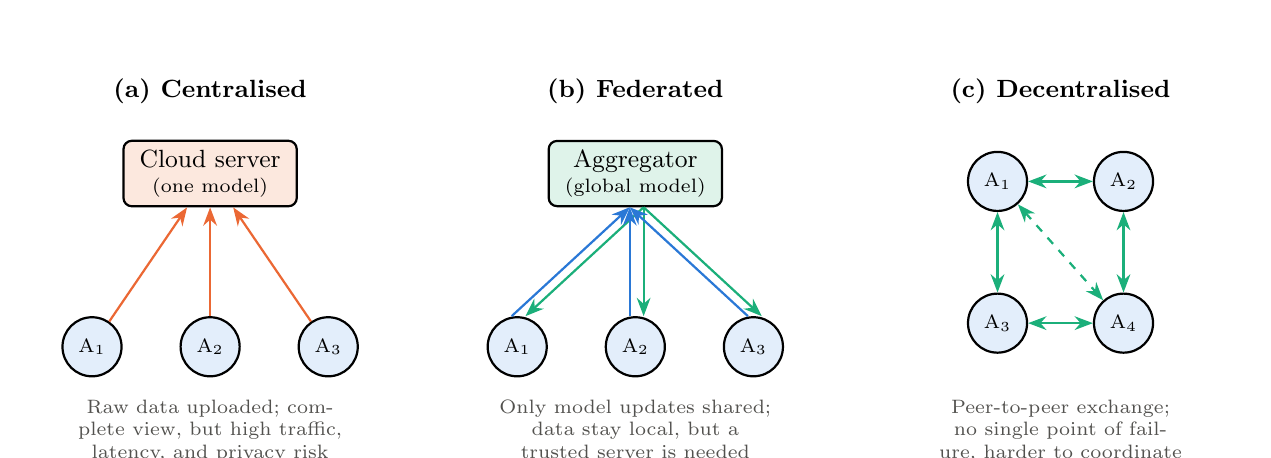
\begin{tikzpicture}[>=Stealth, thick,
  srv/.style={draw, rounded corners=3pt, fill=boxorange, minimum width=2.2cm, minimum height=0.8cm, font=\small, align=center},
  ag/.style={draw, circle, fill=boxblue, minimum size=0.75cm, font=\scriptsize, inner sep=0pt},
  lab/.style={font=\small\bfseries, align=center},
  note/.style={font=\scriptsize, text=inkgray, align=center, text width=4.4cm}]
\node[srv] (s1) at (0,1.6) {Cloud server\\[-2pt]\scriptsize(one model)};
\node[ag] (a11) at (-1.5,-0.6) {A$_1$}; \node[ag] (a12) at (0,-0.6) {A$_2$}; \node[ag] (a13) at (1.5,-0.6) {A$_3$};
\foreach \a in {a11,a12,a13} \draw[->, seriesB] (\a) -- (s1);
\node[lab] at (0,2.65) {(a) Centralised};
\node[note, anchor=north] at (0,-1.15) {Raw data uploaded; complete view, but high traffic, latency, and privacy risk};
\node[srv, fill=boxgreen] (s2) at (5.4,1.6) {Aggregator\\[-2pt]\scriptsize(global model)};
\node[ag] (a21) at (3.9,-0.6) {A$_1$}; \node[ag] (a22) at (5.4,-0.6) {A$_2$}; \node[ag] (a23) at (6.9,-0.6) {A$_3$};
\foreach \a in {a21,a22,a23} {\draw[->, seriesA] ([xshift=-2pt]\a.north) -- ([xshift=-2pt]s2.south); \draw[<-, seriesC] ([xshift=3pt]\a.north) -- ([xshift=3pt]s2.south);}
\node[lab] at (5.4,2.65) {(b) Federated};
\node[note, anchor=north] at (5.4,-1.15) {Only model updates shared; data stay local, but a trusted server is needed};
\node[ag] (a31) at (10.0,1.5) {A$_1$}; \node[ag] (a32) at (11.6,1.5) {A$_2$};
\node[ag] (a33) at (10.0,-0.3) {A$_3$}; \node[ag] (a34) at (11.6,-0.3) {A$_4$};
\draw[<->, seriesC] (a31) -- (a32); \draw[<->, seriesC] (a32) -- (a34); \draw[<->, seriesC] (a34) -- (a33); \draw[<->, seriesC] (a33) -- (a31); \draw[<->, seriesC, dashed] (a31) -- (a34);
\node[lab] at (10.8,2.65) {(c) Decentralised};
\node[note, anchor=north] at (10.8,-1.15) {Peer-to-peer exchange; no single point of failure, harder to coordinate};
\end{tikzpicture}
\caption{Three paradigms for learning across many agents: centralised, federated, and decentralised (peer-to-peer)}
\label{fig:paradigms}
\end{figure}

\paragraph{} At the same time, the \emph{kind} of model being federated has changed. Early work federated supervised predictors; recent work increasingly federates \textbf{decision-making policies}, so that each agent is a reinforcement learner and what is shared is a policy or value network \cite{p1,p2}. Wireless systems are a key application: 6G networks are expected to be ultra-dense, to integrate sensing with communication, to push computation to the edge, and to include aerial nodes, while serving ultra-reliable low-latency (URLLC), enhanced broadband (eMBB), and massive machine-type (mMTC) traffic with very different requirements \cite{p2,p3}.

\section{Motivation}

\paragraph{} Three needs motivate this study. First, \textbf{decentralised decision-making}: vehicular networks change topology every second, edge devices share congested spectrum on limited batteries, and UAV swarms have intermittent connectivity, so a central controller with full observability is unavailable or too slow \cite{p1,p2}. Second, \textbf{privacy and security}: offloading requests reveal location, resource usage reveals behaviour, and traffic used for intrusion detection is confidential; FL keeps these data local, but updates can still leak information and malicious participants can poison the shared model \cite{p2,p3}. Third, \textbf{efficiency}: agents differ in compute, links, and energy, and training that waits for the slowest agent wastes the capacity of the others \cite{p4}.

\section{Problem Statement}

\paragraph{} \emph{Given agents that observe only part of a shared, dynamic environment, hold private data, and differ in their resources, learn policies or models that achieve good collective performance---low latency and energy, high reliability, and fairness---while keeping raw data local, protecting individual updates, and limiting communication and training time.}

\section{Objectives}

\paragraph{} The objectives of this seminar are:
\begin{itemize}
  \item To introduce reinforcement learning, deep and multi-agent RL, and federated learning, on which FedMARL is built.
  \item To review in depth four recent works on federated multi-agent learning for vehicular fog computing, 6G edge resource management, distributed wireless sensing, and decentralised training.
  \item To examine the security and privacy mechanisms used or discussed, including secure aggregation, differential privacy, and defences against poisoning.
  \item To compare the approaches and identify open challenges and future research directions.
\end{itemize}

\section{Scope}

\paragraph{} The seminar covers task offloading in vehicular fog computing \cite{p1}, cross-layer resource management in 6G edge networks \cite{p2}, federated multi-agent learning for sensing, security, and UAV networks as surveyed in \cite{p3}, and workload balancing for serverless training \cite{p4}, together with the algorithms, simulators, datasets, and metrics these works use.

\section{Advantages}

\paragraph{} Federated multi-agent learning offers several advantages over centralised and independent learning:
\begin{itemize}
  \item \textbf{Privacy by Design:} raw data such as positions, traffic, and sensor readings never leave the device.
  \item \textbf{Reduced Communication:} periodic model updates need far less bandwidth than streaming raw data.
  \item \textbf{Faster Convergence:} agents exploring different parts of the environment pool their knowledge.
  \item \textbf{Cross-Domain Applicability:} the same principles apply to vehicles, edge devices, sensors, and UAVs.
\end{itemize}

\section{Organization of the Report}

\paragraph{} \textbf{Chapter 2} introduces the theoretical foundations. \textbf{Chapter 3} reviews the four works in detail. \textbf{Chapter 4} compares the approaches, \textbf{Chapter 5} discusses applications, \textbf{Chapter 6} presents challenges and future directions, and \textbf{Chapter 7} concludes the report.

% ================= CHAPTER 2: THEORETICAL FOUNDATIONS =================
\chapter{Theoretical Foundations}

\paragraph{} This chapter introduces the concepts on which the reviewed works build: reinforcement learning and its deep and multi-agent extensions, federated and decentralised learning, their combination in FedMARL, the privacy and security mechanisms used to protect federated training, the edge-computing context, and the evaluation metrics.

\section{Reinforcement Learning}

\paragraph{} Reinforcement learning formalises sequential decision-making as a \textbf{Markov Decision Process} (MDP), the tuple $\langle\mathcal{S},\mathcal{A},P,r,\gamma\rangle$ of states, actions, transition probabilities $P(s'\mid s,a)$, rewards $r(s,a)$, and discount factor $\gamma\in(0,1]$ \cite{p1}. At each step the agent observes $s_t$, chooses $a_t$ from a policy $\pi(a\mid s)$, receives $r_t$, and moves to $s_{t+1}$. It seeks to maximise the expected discounted return
\begin{equation}
R_t=\sum_{k=0}^{\infty}\gamma^{k}\,r_{t+k}.
\end{equation}
The state value $V^{\pi}(s)=\mathbb{E}_{\pi}[R_t\mid s_t=s]$ and action value $Q^{\pi}(s,a)=\mathbb{E}_{\pi}[R_t\mid s_t=s,a_t=a]$ measure how good a policy is. \textbf{Q-learning} estimates the optimal action value with the temporal-difference (TD) update
\begin{equation}
Q(s_t,a_t)\leftarrow Q(s_t,a_t)+\alpha\Big[r_t+\gamma\max_{a'}Q(s_{t+1},a')-Q(s_t,a_t)\Big],
\end{equation}
where the bracketed term is the \textbf{TD error}. Exploration usually follows an $\epsilon$-greedy rule whose random-action probability decays during training, for example from 1.0 to 0.05 with factor 0.995 in \cite{p2}.

\section{Deep Reinforcement Learning}

\paragraph{} Tables become infeasible when the state space is large, as in vehicular and wireless environments with many queues, positions, and channels \cite{p1}. The \textbf{Deep Q-Network} (DQN) \cite{mnih2015} approximates $Q(s,a;\theta)$ with a neural network and minimises the squared TD error
\begin{equation}
\mathcal{L}(\theta)=\mathbb{E}\Big[\big(r_t+\gamma\max_{a'}Q(s_{t+1},a';\theta^{-})-Q(s_t,a_t;\theta)\big)^{2}\Big],
\end{equation}
where $\theta^{-}$ is a periodically updated \textbf{target network}. Transitions are stored in an \textbf{experience replay} buffer and sampled in mini-batches; \textbf{prioritised replay} samples transitions with large TD error more often \cite{p2}. Under partial observability a single observation is not enough, so the \textbf{Deep Recurrent Q-Network} (DRQN) \cite{hausknecht2015} inserts a Long Short-Term Memory (LSTM) layer that summarises the observation history in a hidden state, $h_t=\mathrm{LSTM}(h_{t-1},o_t)$, and estimates $Q(h_t,a;\theta)$. Paper \cite{p2} gives every agent a DRQN with sequence length 20.

\paragraph{} \textbf{Actor-critic} methods learn the policy $\pi(a\mid s;\theta)$ directly (the \emph{actor}) and use a value network $V(s;w)$ (the \emph{critic}) as a baseline. The actor follows the policy gradient $\nabla_{\theta}\log\pi(a_t\mid s_t;\theta)\,A(s_t,a_t)$, where the \textbf{advantage} with a one-step bootstrap is
\begin{equation}
A(s_t,a_t;\theta,w)=r_t+\gamma V(s_{t+1};w)-V(s_t;w),
\end{equation}
and an \textbf{entropy} bonus $\beta\nabla_{\theta}H(\pi(s_t;\theta))$ keeps the policy exploratory; the critic minimises $A^{2}$ \cite{p1}. The \textbf{Asynchronous Advantage Actor-Critic} (A3C) algorithm \cite{mnih2016} runs several learners in parallel environments, each of which applies its gradients asynchronously to a shared global network and copies the global parameters back. Parallel exploration decorrelates updates, removing the need for replay. This structure---local learners, a shared global model, and asynchronous parameter exchange---is very close to federated learning, which is why paper \cite{p1} builds on it.

\section{Multi-Agent Reinforcement Learning}

\paragraph{} With several learning agents, the MDP generalises to a \textbf{Markov game} in which transitions and each agent's reward depend on the \emph{joint} action. Agents may be cooperative, competitive, or mixed, and homogeneous or heterogeneous. If each agent receives only a local observation $o_i$, the model is a partially observable Markov game, or a \textbf{Decentralised POMDP} (Dec-POMDP) when agents share a team reward \cite{p3}. Paper \cite{p2} formulates 6G resource management as a partially observable multi-agent MDP (POMMDP). In wireless and edge networks, agents map naturally onto network entities---user devices, vehicles, base stations, access points, edge servers, network slices, and UAVs. Their observations include channel state, queue lengths, battery level, age of information, and sensing features, and their actions include transmit power, channel selection, beam choice, trajectory, and offloading decisions. Because these entities share spectrum and compute, one agent's action changes the environment of the others through interference, congestion, and load \cite{p3}. Figure~\ref{fig:marl} illustrates the interaction loop.

\begin{figure}[htbp]
\centering
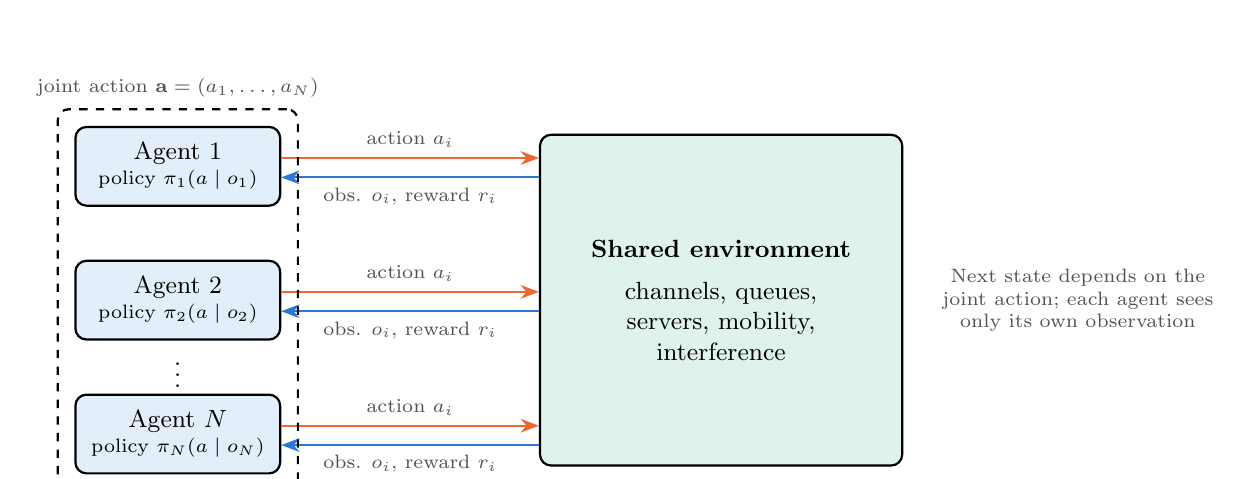
\begin{tikzpicture}[>=Stealth, thick,
  agent/.style={draw, rounded corners=4pt, fill=boxblue, minimum width=2.6cm, minimum height=1.0cm, font=\small, align=center},
  env/.style={draw, rounded corners=4pt, fill=boxgreen, minimum width=4.6cm, minimum height=4.2cm, font=\small, align=center},
  lab/.style={font=\scriptsize, text=inkgray}]
\node[env] (E) at (0,0) {\textbf{Shared environment}\\[4pt]channels, queues,\\ servers, mobility,\\ interference};
\node[agent] (A1) at (-6.9,1.7) {Agent 1\\[-2pt]\scriptsize policy $\pi_1(a\mid o_1)$};
\node[agent] (A2) at (-6.9,0.0) {Agent 2\\[-2pt]\scriptsize policy $\pi_2(a\mid o_2)$};
\node[agent] (AN) at (-6.9,-1.7) {Agent $N$\\[-2pt]\scriptsize policy $\pi_N(a\mid o_N)$};
\node[font=\small] at (-6.9,-0.85) {$\vdots$};
\foreach \a/\y in {A1/1.7,A2/0.0,AN/-1.7} {
  \draw[->, seriesB] ([yshift=3pt]\a.east) -- node[lab, above, pos=0.5]{action $a_i$} ([yshift=3pt]E.west |- 0,\y);
  \draw[<-, seriesA] ([yshift=-4pt]\a.east) -- node[lab, below, pos=0.5]{obs. $o_i$, reward $r_i$} ([yshift=-4pt]E.west |- 0,\y);
}
\node[draw, dashed, rounded corners=4pt, fit=(A1)(AN), inner sep=6pt, label={[font=\scriptsize, text=inkgray]above:joint action $\mathbf{a}=(a_1,\dots,a_N)$}] {};
\node[lab, text width=3.6cm, align=center, anchor=west] at (2.6,0) {Next state depends on the joint action; each agent sees only its own observation};
\end{tikzpicture}
\caption{Multi-agent reinforcement learning under partial observability: every agent acts on local observations, but the environment responds to the joint action}
\label{fig:marl}
\end{figure}

\paragraph{} MARL faces \textbf{non-stationarity} (each agent's environment changes as the others learn), \textbf{scalability} (the joint action space grows exponentially, which \textbf{mean-field} methods address by replacing many neighbours with their average influence), and \textbf{credit assignment} under shared rewards \cite{p3}. A common compromise is \textbf{Centralised Training with Decentralised Execution} (CTDE) \cite{lowe2017}: training may use global information from a simulator or network telemetry, while each agent acts only on its own observations. FedMARL sits between CTDE and fully independent learning: agents learn independently, but periodic model fusion gives them a shared, more global view without centralising data.

\section{Federated Learning}

\paragraph{} Federated learning trains a shared model across $K$ clients whose data remain local. Client $i$ holds $N_i$ samples with local objective $f_i(w)=\frac{1}{N_i}\sum_{n=1}^{N_i}\ell((x_n,y_n);w)$, and the global objective is the data-weighted average \cite{p4}
\begin{equation}
\min_{w}f(w)=\sum_{i=1}^{K}\frac{N_i}{N}f_i(w),\qquad N=\sum_{i=1}^{K}N_i.
\label{eq:flobj}
\end{equation}
The standard algorithm, \textbf{Federated Averaging} (FedAvg) \cite{mcmahan2017}, shown in Algorithm~\ref{alg:fedavg}, alternates local stochastic gradient descent on each client with weighted averaging on the server.

\begin{algorithm}[htbp]
\caption{Federated Averaging (FedAvg)}\label{alg:fedavg}
\begin{algorithmic}[1]
\Require clients $i=1,\dots,K$ with data sizes $N_i$; rounds $R$; local epochs $E$; learning rate $\eta$
\State Initialise global model $w^{0}$
\For{round $r=0$ to $R-1$}
  \State Send $w^{r}$ to a subset $\mathcal{C}_r$ of available clients
  \For{each client $i\in\mathcal{C}_r$ \textbf{in parallel}}
    \State $w_i\gets w^{r}$; run $E$ epochs of $w_i\gets w_i-\eta\nabla f_i(w_i;b)$ over mini-batches $b$
  \EndFor
  \State $w^{r+1}\gets\sum_{i\in\mathcal{C}_r}\frac{N_i}{\sum_{j\in\mathcal{C}_r}N_j}\,w_i$
\EndFor
\State \Return $w^{R}$
\end{algorithmic}
\end{algorithm}

\paragraph{} Real deployments add three complications. \textbf{Statistical heterogeneity}: client data are rarely IID, and non-IID data (often simulated with a Dirichlet distribution, concentration 0.5 in \cite{p4}) make local models drift apart. \textbf{System heterogeneity}: in synchronous FL every round lasts as long as the slowest client, the \textbf{straggler problem}; common remedies select fewer clients, drop the slowest, or vary local work as in FedProx \cite{p4}. \textbf{Communication constraints}: model uploads compete with user traffic for spectrum and power, so client selection, bandwidth and power allocation, and quantisation must be co-designed with learning \cite{p3}. \textbf{Hierarchical FL} aggregates first over short links (for example vehicle to fog) and only occasionally at the cloud, and \textbf{over-the-air computation} lets the wireless channel itself sum simultaneous transmissions, at the cost of fading-induced errors \cite{p1,p3}. Finally, aggregation may be \textbf{synchronous}, with every round waiting for all selected clients, or \textbf{asynchronous}, with the global model updated whenever any client reports. Asynchronous aggregation, used by A3C-style training in \cite{p1}, tolerates slow and intermittently connected clients but must cope with \emph{stale} updates computed from an older global model; synchronous aggregation, used in \cite{p2}, is simpler to analyse and secure but is paced by the slowest participant.

\section{Decentralised and Split Learning}

\paragraph{} \textbf{Decentralised} learning removes the aggregator. In \textbf{gossip learning} agents average with random neighbours; in \textbf{BrainTorrent} they take turns as aggregator; and with \textbf{AllReduce} all agents cooperatively compute the average so that each ends with the same model \cite{p4}. For $K$ agents and a model of $b$ bytes, ring and recursive halving-and-doubling AllReduce both send and receive $2\frac{K-1}{K}b$ bytes per agent, but need $2(K-1)$ and $2\log_2K$ communication steps respectively. \textbf{Split learning} (SL) divides a network at a cut layer so that a weak device trains only the first layers and sends intermediate activations to a stronger party; because classical SL waits for returned gradients in every step, \textbf{local-loss-based split training} attaches a small auxiliary network to the device side so both sides can update in parallel \cite{p4}.

\section{Federated Multi-Agent Reinforcement Learning}

\paragraph{} \textbf{Federated reinforcement learning} applies federated aggregation to RL agents: each agent trains a policy or value network on trajectories it collects locally, and only network parameters are shared \cite{p3}. When the agents also interact in a shared environment, the setting is \textbf{FedMARL} (Figure~\ref{fig:fedmarl}). Its key design choices are \emph{what} is shared (actor-critic weights in \cite{p1}, DRQN weights in \cite{p2}), \emph{when} (every episode in \cite{p1}, every $K$ episodes in \cite{p2}), whether aggregation is synchronous or asynchronous, \emph{who} aggregates (a fog server in \cite{p1}, a server seeing only masked updates in \cite{p2}, all peers via AllReduce in \cite{p4}), and \emph{which} agents participate (only sufficiently charged ones in \cite{p2}).

\begin{figure}[htbp]
\centering
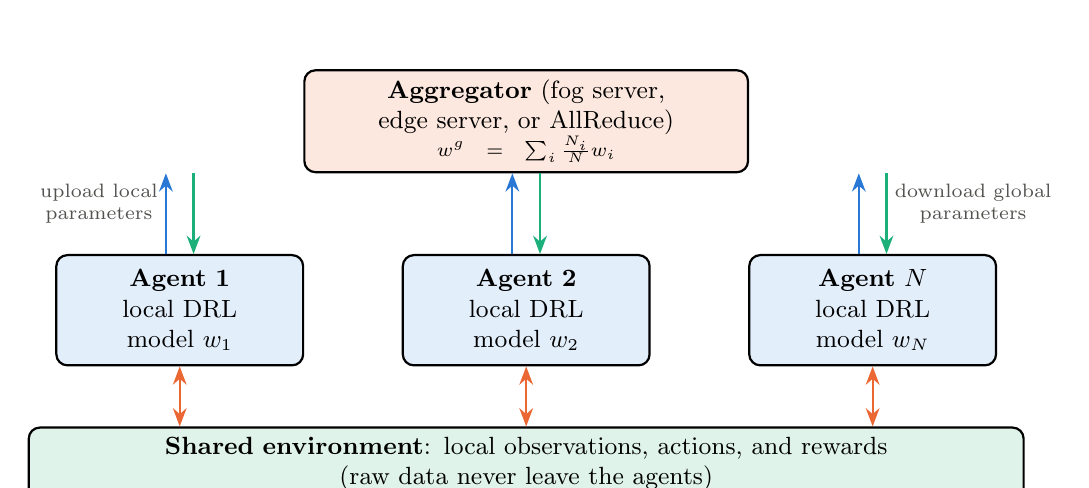
\begin{tikzpicture}[>=Stealth, thick,
  agent/.style={draw, rounded corners=4pt, fill=boxblue, text width=2.9cm, minimum height=1.4cm, font=\small, align=center},
  agg/.style={draw, rounded corners=4pt, fill=boxorange, text width=5.4cm, minimum height=1.0cm, font=\small, align=center},
  envb/.style={draw, rounded corners=4pt, fill=boxgreen, text width=12.4cm, minimum height=0.8cm, font=\small, align=center},
  lab/.style={font=\scriptsize, text=inkgray, align=center}]
\node[agg] (G) at (0,2.9) {\textbf{Aggregator} (fog server, edge server, or AllReduce)\\[-1pt]\scriptsize $w^{g}=\sum_i \frac{N_i}{N} w_i$};
\node[agent] (L1) at (-4.4,0.5) {\textbf{Agent 1}\\ local DRL model $w_1$};
\node[agent] (L2) at (0,0.5) {\textbf{Agent 2}\\ local DRL model $w_2$};
\node[agent] (L3) at (4.4,0.5) {\textbf{Agent $N$}\\ local DRL model $w_N$};
\node[envb] (E) at (0,-1.45) {\textbf{Shared environment}: local observations, actions, and rewards\\ (raw data never leave the agents)};
\foreach \l in {L1,L2,L3} {
  \draw[->, seriesA] ([xshift=-5pt]\l.north) -- ([xshift=-5pt]\l.north |- G.south);
  \draw[<-, seriesC] ([xshift=5pt]\l.north) -- ([xshift=5pt]\l.north |- G.south);
  \draw[<->, seriesB] (\l.south) -- (\l.south |- E.north);
}
\node[lab, anchor=east] at (-4.55,1.85) {upload local\\ parameters};
\node[lab, anchor=west] at (4.55,1.85) {download global\\ parameters};
\end{tikzpicture}
\caption{Federated multi-agent reinforcement learning: agents learn locally from their own interaction and periodically fuse model parameters through an aggregator}
\label{fig:fedmarl}
\end{figure}

\section{Privacy and Security in Federated Learning}

\paragraph{} Keeping data local does not by itself guarantee privacy: \textbf{gradient inversion} and inference attacks can reconstruct samples or attributes from individual updates \cite{p2}. Analyses distinguish a \textbf{semi-honest} adversary, which follows the protocol but learns what it can, from a \textbf{malicious} (Byzantine) one, which may send arbitrary updates. \textbf{Secure aggregation} ensures that the server learns only the \emph{sum} of updates. In the pairwise-masking construction adopted in \cite{p2}, each pair of agents $i<j$ derives a shared secret by elliptic-curve Diffie--Hellman (ECDH) key exchange and expands it into a pseudorandom mask $m_{ij}$; agent $i$ uploads $\tilde{w}_i=w_i+M_i$ with
\begin{equation}
M_i=\sum_{j>i}m_{ij}-\sum_{j<i}m_{ji}.
\end{equation}
Every mask appears once with each sign, so $\sum_iM_i=0$ and the average of masked updates equals the true average (Figure~\ref{fig:secagg}).

\begin{figure}[htbp]
\centering
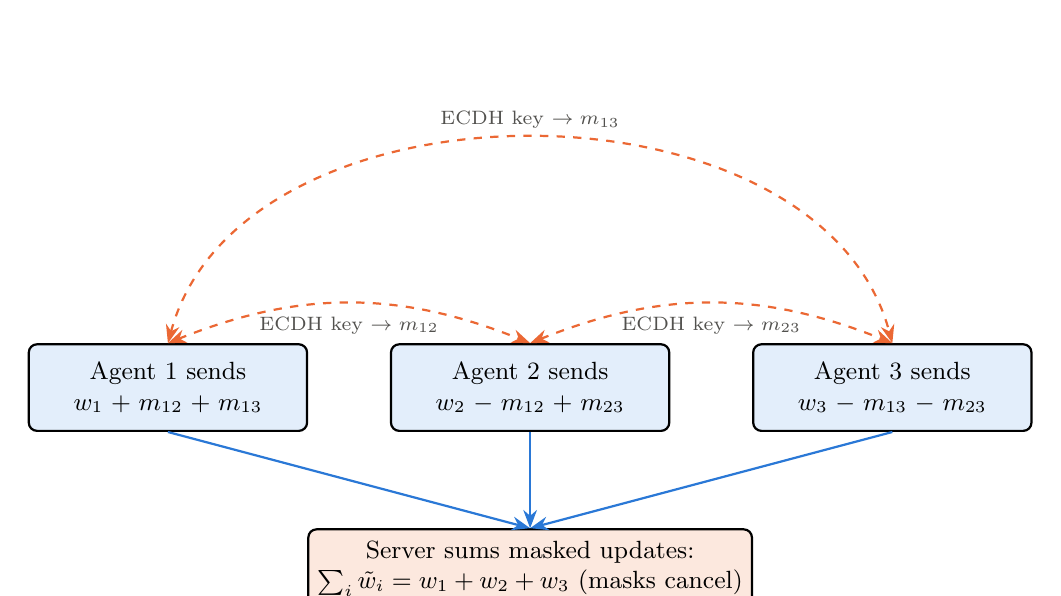
\begin{tikzpicture}[>=Stealth, thick,
  ag/.style={draw, rounded corners=3pt, fill=boxblue, text width=3.3cm, minimum height=1.1cm, font=\small, align=center},
  srv/.style={draw, rounded corners=3pt, fill=boxorange, text width=5.4cm, minimum height=1.0cm, font=\small, align=center},
  lab/.style={font=\scriptsize, text=inkgray, align=center}]
\node[ag] (a1) at (-4.6,0) {Agent 1 sends\\ $w_1+m_{12}+m_{13}$};
\node[ag] (a2) at (0,0) {Agent 2 sends\\ $w_2-m_{12}+m_{23}$};
\node[ag] (a3) at (4.6,0) {Agent 3 sends\\ $w_3-m_{13}-m_{23}$};
\node[srv] (s) at (0,-2.3) {Server sums masked updates:\\ $\sum_i\tilde{w}_i=w_1+w_2+w_3$ (masks cancel)};
\foreach \a in {a1,a2,a3} \draw[->, seriesA] (\a.south) -- (s.north);
\draw[<->, seriesB, dashed] (a1.north) to[bend left=22] node[lab, below=1pt]{ECDH key $\rightarrow m_{12}$} (a2.north);
\draw[<->, seriesB, dashed] (a2.north) to[bend left=22] node[lab, below=1pt]{ECDH key $\rightarrow m_{23}$} (a3.north);
\draw[<->, seriesB, dashed] (a1.north) to[out=75,in=105] node[lab, above]{ECDH key $\rightarrow m_{13}$} (a3.north);
\end{tikzpicture}
\caption{Secure aggregation with pairwise masks: each individual upload is hidden, but the masks cancel in the sum}
\label{fig:secagg}
\end{figure}

\paragraph{} \textbf{Differential privacy} (DP) gives a statistical guarantee: a mechanism $\mathcal{M}$ is $(\epsilon,\delta)$-differentially private if, for datasets $D,D'$ differing in one record and any output set $S$, $\Pr[\mathcal{M}(D)\in S]\le e^{\epsilon}\Pr[\mathcal{M}(D')\in S]+\delta$. It is achieved by clipping updates and adding noise; paper \cite{p4} evaluates Laplace-noise DP with $\epsilon=0.5$, $\delta=10^{-5}$. Malicious participants can instead mount \textbf{data or model poisoning} and \textbf{backdoor} attacks, and multi-agent RL systems can also be attacked by observation spoofing and reward manipulation \cite{p3}. Defences include robust aggregation, anomaly detection, and trust scores---but secure aggregation, by hiding individual updates, also hides the evidence needed to detect poisoned ones.

\section{Edge Computing and Wireless Context}

\paragraph{} \textbf{Mobile edge computing} (MEC) places compute at base stations so devices can offload computation with low latency. In \textbf{vehicular fog computing}, tasks from moving vehicles can run locally, on neighbouring vehicles (V2V), on parked vehicles (V2P), or on roadside fog servers \cite{p1}. The offloading decision balances transmission delay, bounded by the link capacity $C=B\log_2(1+P_t\,l/N_0)$ for bandwidth $B$, power $P_t$, path-loss factor $l$, and noise $N_0$, against queuing and computation delay at the destination. With Poisson arrivals at rate $\lambda$ and service rate $\mu$, queuing delay grows sharply as $\lambda/\mu$ approaches one, so a task's \textbf{residence time} is highly sensitive to load \cite{p1}. In 6G, URLLC, eMBB, and mMTC tasks compete through the \textbf{Medium Access Control} (MAC) layer, and offloading, channel selection, and CPU speed interact, motivating \textbf{cross-layer} optimisation \cite{p2}. 6G will also include \textbf{UAV-enabled} networks, in which trajectory becomes a control variable coupled with power and multiple access, and \textbf{integrated sensing and communication} (ISAC) \cite{p3}. Table~\ref{tab:services} lists the three 6G service classes with the task sizes and deadlines used to simulate them in \cite{p2}.

{\renewcommand{\arraystretch}{1.2}
\begin{table}[htbp]
\centering
\caption{6G service classes and the task profiles used to simulate them in \cite{p2}}\label{tab:services}
\small
\begin{tabularx}{\textwidth}{|p{2.0cm}|X|p{1.7cm}|p{1.7cm}|}
\hline
\textbf{Class} & \textbf{Characteristics and example applications} & \textbf{Task size} & \textbf{Deadline} \\ \hline
URLLC & Ultra-reliable, very low latency; autonomous driving, industrial control & 1 MB & 2 s \\ \hline
eMBB & High data rate; video streaming, augmented and virtual reality & 3 MB & 5 s \\ \hline
mMTC & Many low-power devices with small, delay-tolerant messages; IoT sensing & 0.5 MB & 10 s \\ \hline
\end{tabularx}
\end{table}}

\section{Evaluation Metrics}

\paragraph{} Table~\ref{tab:metrics} summarises the metrics used by the reviewed works. Fairness is measured with \textbf{Jain's index} over per-agent allocations $x_i$,
\begin{equation}
F_{\mathrm{Jain}}=\frac{\big(\sum_{i=1}^{N}x_i\big)^{2}}{N\sum_{i=1}^{N}x_i^{2}}\in\Big[\frac{1}{N},1\Big],
\label{eq:jain}
\end{equation}
which equals 1 for equal allocations and $1/N$ when one agent receives everything.

{\renewcommand{\arraystretch}{1.15}
\begin{table}[htbp]
\centering
\caption{Evaluation metrics used in the reviewed works}\label{tab:metrics}
\small
\begin{tabularx}{\textwidth}{|p{3.4cm}|X|p{1.3cm}|}
\hline
\textbf{Metric} & \textbf{Definition} & \textbf{Used in} \\ \hline
Residence time & Time a task spends queued and executing & \cite{p1} \\ \hline
End-to-end delay & Transmission + queuing + computation delay & \cite{p1} \\ \hline
Delivery / utilisation ratio & Results returned per task offloaded; tasks computed per task received & \cite{p1} \\ \hline
Reliability & Rolling fraction of tasks completed within their deadline & \cite{p2} \\ \hline
Energy per task; energy efficiency & Joules per task; throughput per joule (bits/J) & \cite{p2} \\ \hline
Spectral efficiency & Throughput per unit bandwidth (bps/Hz) & \cite{p2} \\ \hline
Fairness & Jain's index, optionally combined with channel-access entropy & \cite{p2} \\ \hline
Scalability & Performance retained as the number of agents grows & \cite{p2,p4} \\ \hline
Training time to target accuracy & Wall-clock time until the global model reaches a set accuracy & \cite{p4} \\ \hline
\end{tabularx}
\end{table}}

\section{Taxonomy of Approaches}

\paragraph{} Following the survey \cite{p3}, federated multi-agent learning can be classified by its learning formulation, training topology, agent model, and application domain. Figure~\ref{fig:taxonomy} shows this taxonomy and the complementary positions of the four reviewed works.

\begin{figure}[htbp]
\centering
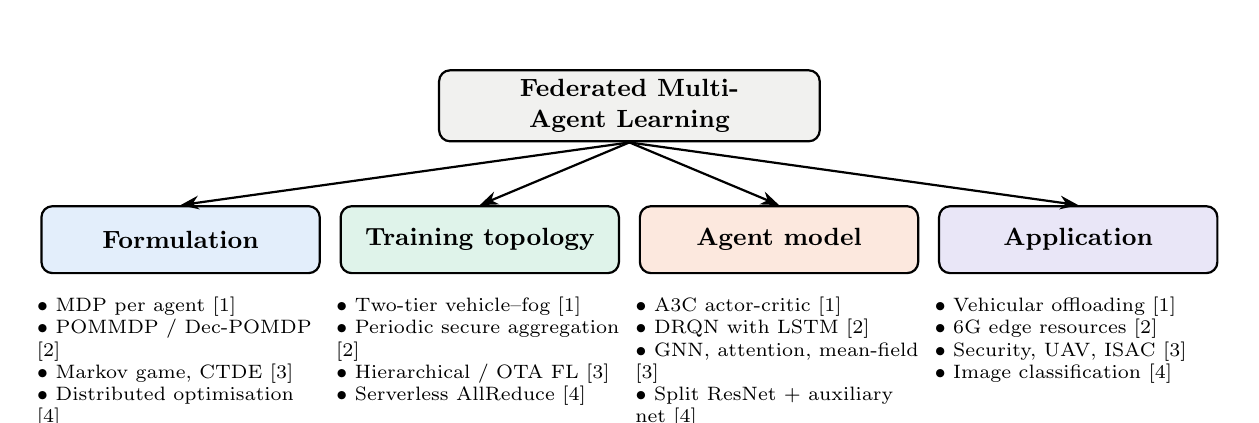
\begin{tikzpicture}[>=Stealth, thick,
  root/.style={draw, rounded corners=4pt, fill=boxgray, text width=4.6cm, minimum height=0.9cm, font=\small\bfseries, align=center},
  cat/.style={draw, rounded corners=4pt, text width=3.3cm, minimum height=0.85cm, font=\small\bfseries, align=center},
  leaf/.style={font=\scriptsize, align=left, text width=3.65cm, anchor=north}]
\node[root] (R) at (0,0) {Federated Multi-Agent Learning};
\node[cat, fill=boxblue]   (c1) at (-5.7,-1.7) {Formulation};
\node[cat, fill=boxgreen]  (c2) at (-1.9,-1.7) {Training topology};
\node[cat, fill=boxorange] (c3) at (1.9,-1.7)  {Agent model};
\node[cat, fill=boxviolet] (c4) at (5.7,-1.7)  {Application};
\foreach \c in {c1,c2,c3,c4} \draw[->] (R.south) -- (\c.north);
\node[leaf] at (-5.7,-2.3) {$\bullet$ MDP per agent [1]\\ $\bullet$ POMMDP / Dec-POMDP [2]\\ $\bullet$ Markov game, CTDE [3]\\ $\bullet$ Distributed optimisation [4]};
\node[leaf] at (-1.9,-2.3) {$\bullet$ Two-tier vehicle--fog [1]\\ $\bullet$ Periodic secure aggregation [2]\\ $\bullet$ Hierarchical / OTA FL [3]\\ $\bullet$ Serverless AllReduce [4]};
\node[leaf] at (1.9,-2.3)  {$\bullet$ A3C actor-critic [1]\\ $\bullet$ DRQN with LSTM [2]\\ $\bullet$ GNN, attention, mean-field [3]\\ $\bullet$ Split ResNet + auxiliary net [4]};
\node[leaf] at (5.7,-2.3)  {$\bullet$ Vehicular offloading [1]\\ $\bullet$ 6G edge resources [2]\\ $\bullet$ Security, UAV, ISAC [3]\\ $\bullet$ Image classification [4]};
\end{tikzpicture}
\caption{A taxonomy of federated multi-agent learning and the positions of the reviewed works}
\label{fig:taxonomy}
\end{figure}

\paragraph{} The taxonomy shows that the works are complementary rather than competing. The two reinforcement learning frameworks \cite{p1,p2} differ mainly in agent model and coordination: an online actor-critic with asynchronous two-tier aggregation for fast-changing vehicular networks, versus a recurrent value-based agent with periodic secure aggregation for partially observable 6G edge networks. ComDML \cite{p4} addresses the training process that both depend on, and the survey \cite{p3} places all three within a wider space of formulations, architectures, and applications that includes network security and UAV control.

\section{Chapter Summary}

\paragraph{} This chapter introduced the MDP formulation of RL and its deep (DQN, DRQN, actor-critic, A3C) and multi-agent (Markov game, Dec-POMDP, CTDE) extensions; federated, decentralised, and split learning and their combination with RL; secure aggregation, differential privacy, and poisoning threats; the vehicular, 6G, and UAV settings; and the evaluation metrics. The next chapter uses these concepts to review the four selected works.

% ================= CHAPTER 3: LITERATURE SURVEY =================
\chapter{Literature Survey}

\paragraph{} This chapter reviews the four selected works. For each, the problem, formulation, algorithm, experimental setup, and principal results are presented, followed by a brief critical discussion. The base paper \cite{p1} is reviewed first, followed by FERMI-6G \cite{p2}, the survey \cite{p3}, and ComDML \cite{p4}.

% ---------------------------------------------------------------
\section{A Federated Multi-Agent Deep Reinforcement Learning for Vehicular Fog Computing}

\paragraph{} Shabir, Rahman, Malik, Buyya, and Khan \cite{p1}, in \textit{The Journal of Supercomputing}, propose a two-tier federated multi-agent DRL framework that learns task-offloading decisions in vehicular fog computing: vehicles train local actor-critic models, and a federation of fog servers aggregates them into a global model.

\subsection{Problem Statement and Motivation}

\paragraph{} Vehicular fog computing lets moving vehicles use the idle resources of neighbouring vehicles, parked vehicles, and roadside fog servers. Choosing \emph{where} each task runs is hard because topology, arrival rates, and queue states change continuously \cite{p1}. Heuristics, game theory, bandits, and genetic algorithms consider few parameters or need centralised management and degrade under heavy load, while single-agent or centralised DRL converges slowly to local optima because each learner sees little of the environment. Sharing raw state is also costly and privacy-invasive. The paper asks whether federating the learning---training on each vehicle and sharing only parameters with the fog tier---gives faster convergence and better offloading with less communication and more privacy.

\subsection{System Model and Problem Formulation}

\paragraph{} The environment contains moving vehicles $\mathcal{V}$, parked vehicles $\mathcal{P}$, and fog servers $\mathcal{F}$; only moving vehicles generate tasks. The path loss at distance $d$ is $l=a+\beta\log_{10}(d)+b$ (offset $a$, shadow fading $b$, attenuation index $\beta$), and the channel is assumed quasi-static and homogeneous. Each task $j$ has size $s_j$ (MB) and computing requirement $c_j$ (Mbits). Nodes are multi-server FIFO queues with Poisson arrivals at rate $\lambda$, and the \textbf{residence time} of agent $i$ with clock frequency $f_i$ and queue $Q$ is
\begin{equation}
Z_i=\frac{\sum_{x\in Q}c_x}{f_i}.
\end{equation}
The service time of a task is $D_i=D^{1}_i+D^{2}_i+D^{3}_i$, the sum of the transmission delay $D^{1}_i=\psi_iB(D^{\uparrow}_i+D^{\downarrow}_i)$ weighted by the frequency-reuse cost $\psi_i$, the computation delay $D^{2}_i=(\psi_2f_i)\sum_jc_j/f_i$ with unit lease cost $\psi_2$, and the queuing delay $D^{3}_i=(\psi_2f_i)\sum_jZ_j$ \cite{p1}.

\paragraph{} Each vehicle is an agent with state
\begin{equation}
S_i=\{Z_i,\ \Delta_i,\ V_i,\ W_i,\ f_i,\ (s_j,c_j)\},
\end{equation}
containing the residence times of, distances to, relative speeds of, and offloading modes of the available resources, the agent's own capacity, and the task attributes. The action space $A_i=\{a_1,a_2,a_3,a_4\}$ executes the task locally or offloads it to a moving vehicle, a fog server, or a parked vehicle. The reward for executing at destination $k$ is
\begin{equation}
r_i=-\frac{1}{\lambda}\,Z_k ,
\end{equation}
so destinations with shorter queues earn more reward. The objective is to minimise the expected discounted value, which corresponds to task waiting time, subject to binary decisions and workload not exceeding capacity \cite{p1}.

\subsection{Multi-Agent A3C and Two-Tier Federation}

\paragraph{} Each agent learns with A3C (Section~2.2). With advantage $A(s_t,a_i;\theta,w)=r_t+\gamma V(s_{t+1};w)-V(s_t;w)$, the actor and critic gradients are
\begin{equation}
d\theta\leftarrow d\theta+\nabla_{\theta}\log\pi_{\theta}(a_i\mid s_t)\,A+\beta\nabla_{\theta}H\big(\pi(s_t;\theta)\big),\qquad dw\leftarrow dw+\frac{\partial A^{2}}{\partial w},
\end{equation}
where the entropy term prevents premature convergence \cite{p1}. Learning is \textbf{online}: parallel environments generate fresh experience, which suits a setting for which no complete dataset exists.

\begin{figure}[htbp]
\centering
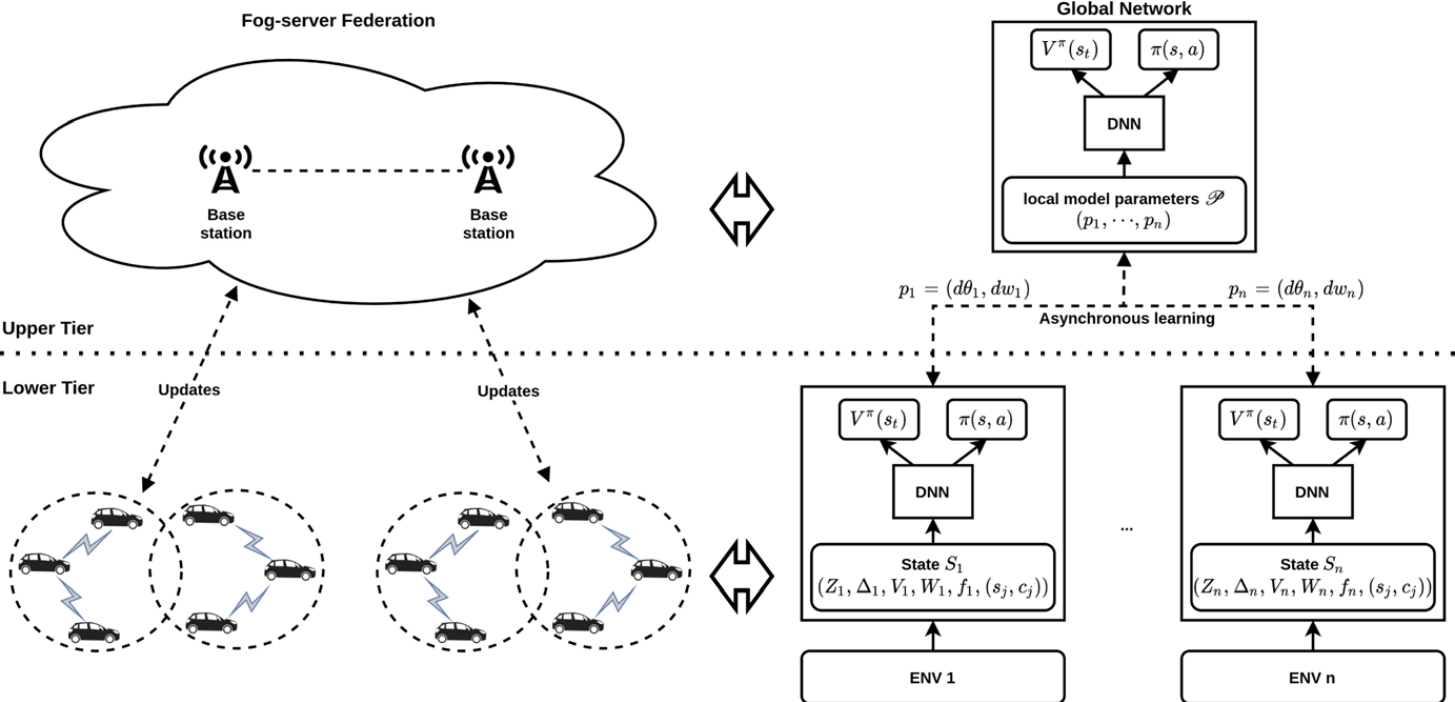
\includegraphics[width=0.88\textwidth]{figs/p1_architecture.png}
\caption{Two-tier federated learning framework: vehicles in the lower tier train local actor-critic models, and the fog-server federation in the upper tier maintains the global network \cite{p1}}
\label{fig:p1_arch}
\end{figure}

\paragraph{} Figure~\ref{fig:p1_arch} shows the architecture. In the \textbf{lower tier}, each vehicle initialises its local actor-critic from the global network, learns online for up to $t_{\max}$ steps, and computes policy and value gradients. In the \textbf{upper tier}, local weights are sent after every episode to a federation of fog servers; one under-loaded server, $\arg\min_{i\in\mathcal{F}}Z_i$, is delegated to maintain the global network, which aggregates the local models asynchronously and returns the result (Algorithm~\ref{alg:p1}). The fog tier connects to many more vehicles than any single vehicle does, so it gives each agent a wider view of the environment, while only model parameters cross the network \cite{p1}.

\begin{algorithm}[htbp]
\caption{Two-tier federated A3C task offloading (summarised from \cite{p1})}\label{alg:p1}
\begin{algorithmic}[1]
\Require vehicles $\mathcal{V}$ with local networks $(\theta_i,w_i)$; fog federation $\mathcal{F}$; episode length $t_{\max}$
\State Delegate fog server $f^{*}\gets\arg\min_{f\in\mathcal{F}}Z_f$ to host the global network $(\theta,w)$
\For{each episode}
  \For{each vehicle $i\in\mathcal{V}$ \textbf{in parallel}}
    \State $(\theta_i,w_i)\gets(\theta,w)$
    \For{$t=1$ to $t_{\max}$}
      \State Build $S_i$ on task arrival; choose $a_i\sim\pi(a\mid S_i;\theta_i)$ among local, vehicle, fog, parked
      \State Execute at destination $k$; observe reward $r_i=-Z_k/\lambda$
    \EndFor
    \State Compute advantage, policy loss with entropy, and value loss; send $(d\theta_i,dw_i)$ to $\mathcal{F}$
  \EndFor
  \State $f^{*}$ aggregates updates asynchronously into $(\theta,w)$ and returns the global model
\EndFor
\end{algorithmic}
\end{algorithm}

\subsection{Experimental Setup}

\paragraph{} The framework is simulated in SUMO on a Manhattan grid of 900 m $\times$ 900 m for 1000 time steps with 100 moving vehicles, 20 parked vehicles, and 9 fog servers. Vehicle and fog clocks are 0.6--1.0 GHz and 2.0 GHz, transmission ranges 100 m and 200 m, and V2V, V2R, and V2P bandwidths 1, 2, and 1 MHz; tasks need 0.2--1.0 Mbits of computation and carry 1--6 MB of data. The actor-critic network has layers of 32, 16, 8, and 4 neurons with tanh and softmax activations and the Adam optimiser (learning rate $10\mathrm{e}{-5}$, discount 0.955), implemented in TensorFlow 1.13.1 with two parallel simulation threads. Arrival rates range from $\lambda=60$ to 200 tasks/s. Baselines are the \textbf{Stochastic Selection Algorithm} (SA), which picks a destination uniformly at random within range, and the \textbf{Greedy Algorithm} (GA), which picks the nearest node \cite{p1}.

\subsection{Results and Analysis}

\paragraph{} \textbf{Delay and cost.} At low load all methods behave alike, but beyond $\lambda=140$ GA and SA overload some nodes while the DRL scheme spreads the load (Figure~\ref{fig:p1_delay}). At $\lambda=200$ it reduces residence time by \textbf{58.6\%} and end-to-end delay by \textbf{57.11\%}, while SA and GA incur 16\% and 56\% higher system cost \cite{p1}. GA has the lowest \emph{transmission} delay because it always offloads to the nearest node, which is exactly what creates its long queues; the DRL agent accepts longer transmissions when a farther node has a much shorter queue.

\begin{figure}[htbp]
\centering
\begin{subfigure}[t]{0.45\textwidth}\centering
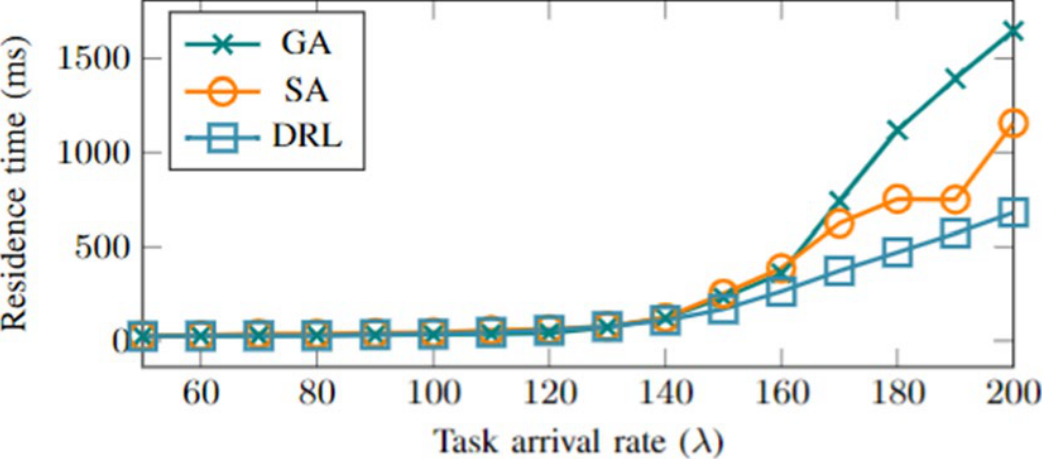
\includegraphics[width=\linewidth]{figs/p1_residence.png}
\caption{Mean residence time}
\end{subfigure}\hfill
\begin{subfigure}[t]{0.45\textwidth}\centering
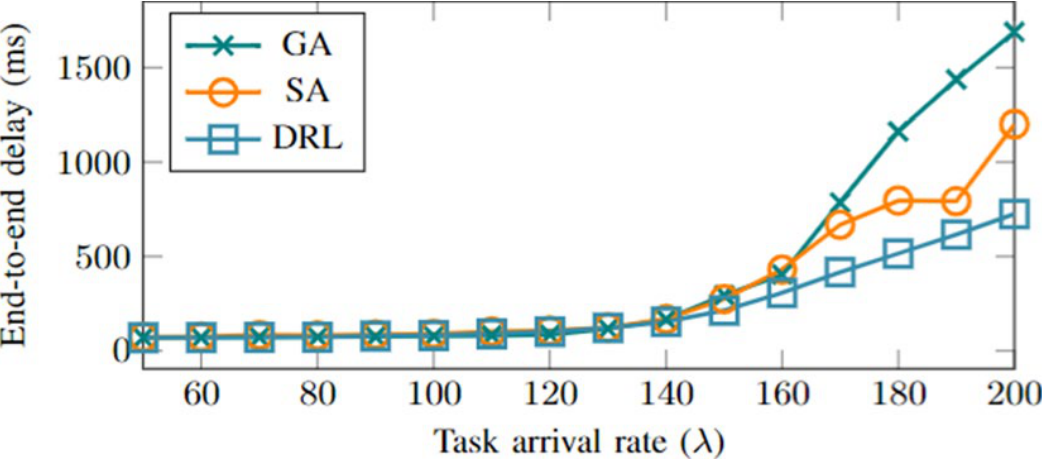
\includegraphics[width=\linewidth]{figs/p1_e2e.png}
\caption{Mean end-to-end delay}
\end{subfigure}
\caption{Residence time and end-to-end delay versus task arrival rate for GA, SA, and the proposed DRL scheme \cite{p1}}
\label{fig:p1_delay}
\end{figure}

\paragraph{} \textbf{Delivery and failures.} The delivery rate of GA and SA drops by 45.9\% and 20.4\% at $\lambda=200$, while the DRL scheme stays highest (Figure~\ref{fig:p1_delivery}). It delivers about 15{,}000 tasks, 8{,}817 of them in a single hop---the most first-hop deliveries of the three methods---and records 13{,}844 failures against 20{,}535 for SA and 43{,}679 for GA, a reduction the authors summarise as 69\% relative to GA \cite{p1}.

\begin{figure}[htbp]
\centering
\begin{subfigure}[t]{0.45\textwidth}\centering
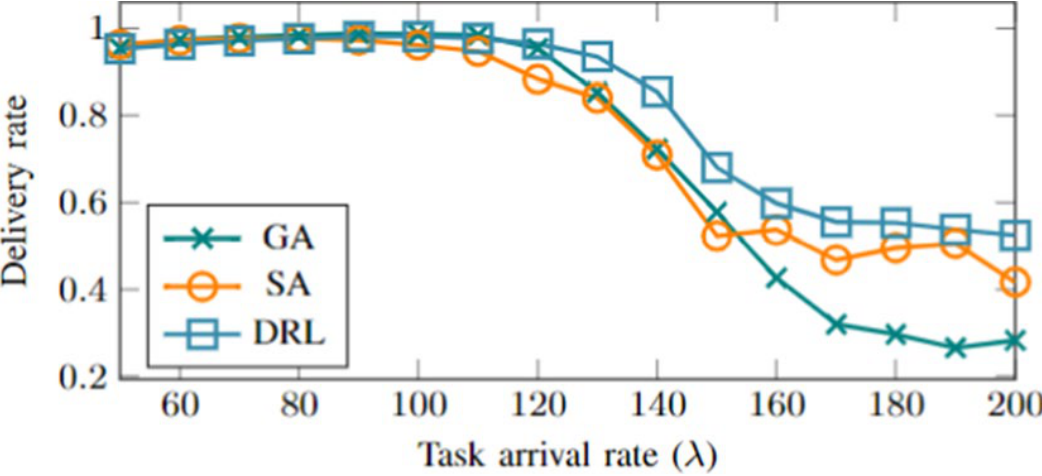
\includegraphics[width=\linewidth]{figs/p1_delivery.png}
\caption{Result delivery ratio}
\end{subfigure}\hfill
\begin{subfigure}[t]{0.45\textwidth}\centering
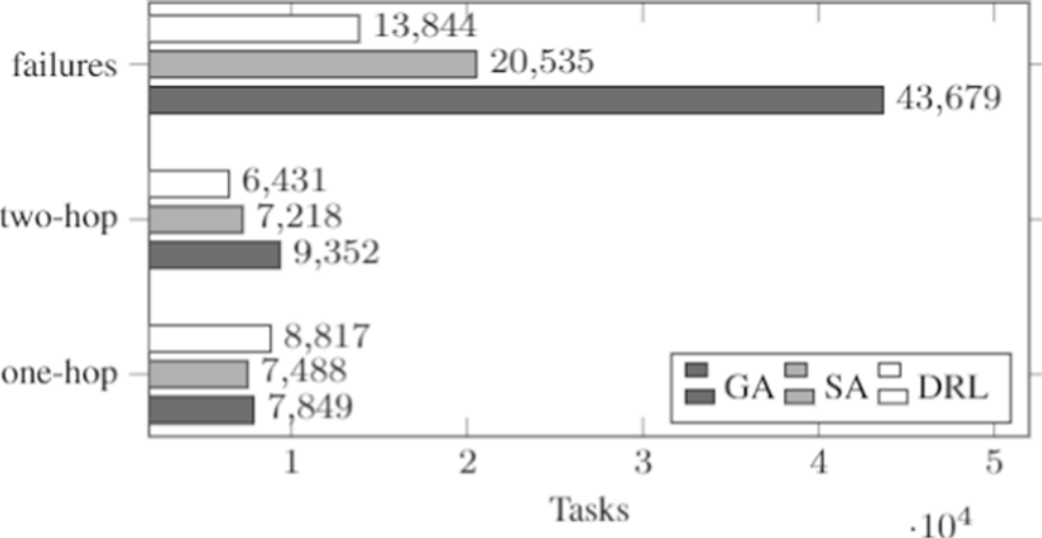
\includegraphics[width=\linewidth]{figs/p1_delivstats.png}
\caption{Task delivery statistics at $\lambda=200$}
\end{subfigure}
\caption{Delivery ratio versus arrival rate, and one-hop deliveries, two-hop deliveries, and failures at $\lambda=200$ \cite{p1}}
\label{fig:p1_delivery}
\end{figure}

\paragraph{} \textbf{Workload and utilisation.} The DRL scheme executes the most tasks locally (96{,}482 against 92{,}505 for SA and 67{,}826 for GA, reported as a 30\% gain over GA) and spreads the rest almost evenly, about 14{,}500 each, over moving vehicles, fog servers, and parked vehicles, whereas GA sends 41{,}081 tasks to neighbouring vehicles (Figure~\ref{fig:p1_util}). It achieves the highest utilisation ratio, improving V2P by 5.35\% and V2V by 8.5\%. Actor and critic losses settle after about $10^{4}$ iterations, confirming convergence \cite{p1}.

\begin{figure}[htbp]
\centering
\begin{subfigure}[t]{0.45\textwidth}\centering
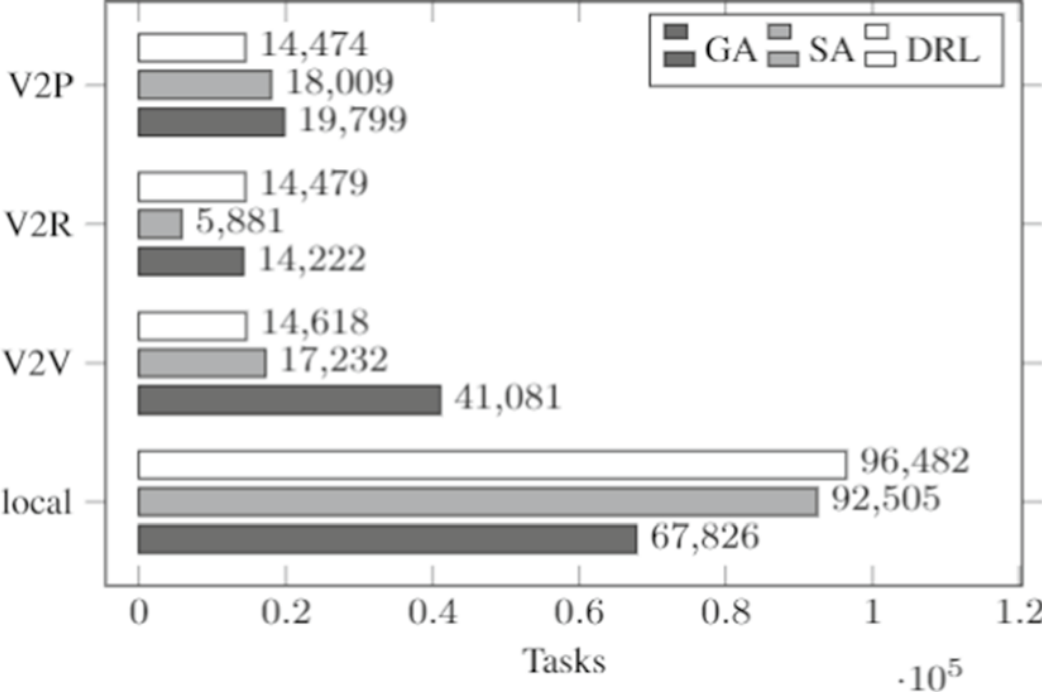
\includegraphics[width=\linewidth]{figs/p1_taskstats.png}
\caption{Tasks allocated per destination}
\end{subfigure}\hfill
\begin{subfigure}[t]{0.45\textwidth}\centering
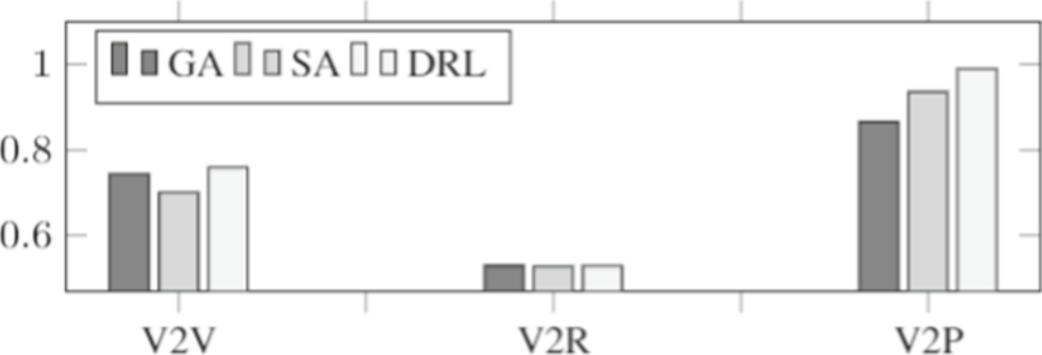
\includegraphics[width=\linewidth]{figs/p1_utilization.png}
\caption{Utilisation ratio}
\end{subfigure}
\caption{Workload distribution and utilisation ratio at $\lambda=200$ tasks/s \cite{p1}}
\label{fig:p1_util}
\end{figure}

\subsection{Discussion}

\paragraph{} The paper combines multi-agent DRL, asynchronous A3C, and two-tier vehicle--fog federation in a practical framework with large gains under heavy load, and its residence-time reward is simple and well aligned with the goal of avoiding congested nodes. Its limitations are that the baselines are simple heuristics, the channel is assumed homogeneous and quasi-static, only two training threads were used, and---as the authors acknowledge---updates are shared in plain form, leaving the system open to gradient spoofing and inference attacks. These gaps are addressed by the secure aggregation of FERMI-6G \cite{p2} and the communication-efficient training of ComDML \cite{p4}.

% ---------------------------------------------------------------
\section{Federated Multi-Agent Reinforcement Learning for Privacy-Preserving and Energy-Aware Resource Management in 6G Edge Networks}

\paragraph{} Andong and Min \cite{p2} propose \textbf{FERMI-6G} (Federated Energy-aware Reinforcement for Multi-agent Intelligence in 6G), in which edge agents jointly decide task offloading, spectrum access, and CPU frequency and synchronise through cryptographic secure aggregation.

\subsection{Problem Statement and Motivation}

\paragraph{} Ultra-dense, energy-constrained 6G networks must serve URLLC, eMBB, and mMTC traffic. Centralised resource management suffers from scalability bottlenecks, signalling overhead, and privacy risk, existing MARL solutions often assume full observability and optimise one metric at one layer, and standard FL is vulnerable to gradient inversion \cite{p2}. FERMI-6G aims to be decentralised, private, energy-aware, and cross-layer under partial observability and mobility.

\subsection{System Model and Reward}

\paragraph{} At each interval, agent $i$ selects a composite \textbf{cross-layer action}
\begin{equation}
a_i(t)=\big(a^{\mathrm{app}}_i(t),\ a^{\mathrm{mac}}_i(t),\ a^{\mathrm{cpu}}_i(t)\big),
\end{equation}
choosing local execution or offloading ($a^{\mathrm{app}}_i\in\{0,1\}$), a channel ($a^{\mathrm{mac}}_i\in\{1,\dots,k\}$), and a CPU frequency ($a^{\mathrm{cpu}}_i\in\mathbb{R}$). The environment is a POMMDP in which agent $i$ observes only $o_i(t)=\{q_i,E_i,h_i,\lambda_i,c_i\}$: queue, residual energy, channel gain, task type, and CPU usage \cite{p2}. Each agent uses a DRQN with prioritised replay (Figure~\ref{fig:p2_arch}).

\begin{figure}[htbp]
\centering
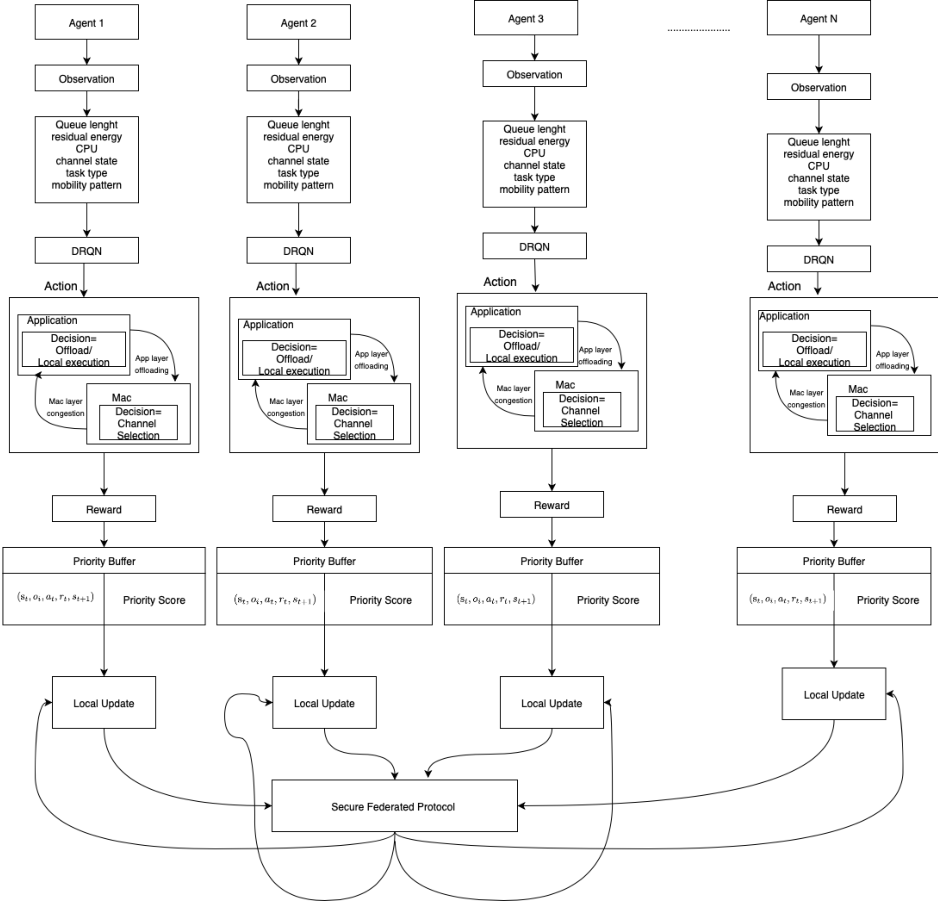
\includegraphics[width=0.52\textwidth]{figs/p2_architecture.png}
\caption{System architecture of FERMI-6G: each agent observes local state, selects application- and MAC-layer actions with a DRQN, stores prioritised experience, updates locally, and joins the secure federated protocol \cite{p2}}
\label{fig:p2_arch}
\end{figure}

\paragraph{} The reward combines normalised latency $\tilde{L}_i=L_i/D_i$ (latency over deadline), normalised energy per task $\tilde{E}_i=E_i/E_{\max}$, a \textbf{hybrid fairness} index $F_i=\beta_{\mathrm{jain}}F_{\mathrm{Jain}}+\beta_{\mathrm{entropy}}H_{\mathrm{avg}}$ that mixes Jain's index (Equation~\ref{eq:jain}) with the average normalised channel-access entropy, reliability $R_i$ (a rolling task-success average), spectral efficiency, energy efficiency, and MAC success rate:
\begin{equation}
\begin{split}
r_i(t)={}&w_L\tilde{L}^{-1}_iP_{\mathrm{dyn}}+w_E\tilde{E}^{-1}_iP_{\mathrm{energy}}+w_FF_i+w_RR_i\\
&+w_{SE}\widetilde{SE}_i+w_{EE}EE_i+w_{MAC}\,\mathrm{MAC}_{\mathrm{rate},i},
\end{split}
\end{equation}
where the penalties $P_{\mathrm{dyn}}$ and $P_{\mathrm{energy}}$ double the latency and energy terms when latency exceeds 2 s or energy falls below a threshold \cite{p2}. The reward is also decomposed into application-layer (latency and computation energy) and MAC-layer (transmission energy and fairness) components so that agents learn how the two layers interact.

\subsection{Secure Aggregation and the FERMI-6G Algorithm}

\paragraph{} Every $K$ episodes, agents synchronise with the pairwise-masking protocol of Section~2.7, adapted from Google's secure aggregation framework \cite{bonawitz2017} to federated MARL: masks derived from ECDH keys and AES cancel in the sum, so the aggregator recovers the exact average without seeing any individual model under a semi-honest adversary. Only agents whose energy exceeds $E_{\mathrm{threshold}}$ take part in a round \cite{p2}. The global objective maximises long-term reward subject to minimum energy per agent, partial observability, and a communication budget. FERMI-6G's four innovations are temporal DRL with LSTM-based DRQNs, the cross-layer action space, secure synchronisation, and optional adaptive reward weights driven by moving averages of system metrics. Algorithm~\ref{alg:p2} condenses the method.

\begin{algorithm}[htbp]
\caption{FERMI-6G local learning and secure aggregation (condensed from \cite{p2})}\label{alg:p2}
\begin{algorithmic}[1]
\Require agents $\mathcal{A}$ with DRQN $\theta_i$, target $\theta^{\mathrm{target}}_i$, replay $B_i$, ECDH keys; episodes $N$; steps $T$; interval $K$
\For{episode $n=1$ to $N$}
  \For{$t=1$ to $T$, for each agent $i$}
    \State $h_i\gets\mathrm{LSTM}(h_i,o_i(t))$; select $a_i=(a^{\mathrm{app}}_i,a^{\mathrm{mac}}_i,a^{\mathrm{cpu}}_i)$ $\epsilon$-greedily from $Q(h_i,\cdot\,;\theta_i)$
    \State Execute; store $(h_i,a_i,r_i,o_i(t+1))$ with priority; update $\theta_i$ on a prioritised mini-batch
  \EndFor
  \If{$n \bmod K=0$}
    \State Each agent with $E_i>E_{\mathrm{threshold}}$ sends $\theta_i+M_i$ with $M_i=\sum_{j>i}m_{ij}-\sum_{j<i}m_{ji}$
    \State Aggregator broadcasts $\theta_g=\frac{1}{|\mathcal{A}|}\sum_i(\theta_i+M_i)$; agents set $\theta_i,\theta^{\mathrm{target}}_i\gets\theta_g$
    \State (Optional) adapt and renormalise reward weights
  \EndIf
\EndFor
\end{algorithmic}
\end{algorithm}

\subsection{Experimental Setup}

\paragraph{} Agents move by random walk (0.1--1.0 m/s) on a $100\times100$ grid with the edge server at $[50,50]$. Tasks are URLLC (1 MB, 2 s deadline), eMBB (3 MB, 5 s), or mMTC (0.5 MB, 10 s); batteries must stay above 20\%; the MAC layer models congestion, collisions, and retransmissions (probability 30\%). Training runs 800 episodes of 20 steps with 5 agents, a 10{,}000-transition buffer, batch size 16, $\gamma=0.99$, learning rate $10^{-3}$, and sequence length 20 on a 2016 laptop \cite{p2}. Four frameworks are compared: \textbf{FERMI-6G}; \textbf{Fed-MARL}, the same federated framework without cross-layer learning (its MAC and CPU decisions are made by heuristics, which raised its reliability from about 30\% to about 94\%); \textbf{Centralised RL} with a single-layer policy; and \textbf{Centralised RL (Cross-Layer)}. Because the centralised frameworks obtained rewards near $-147$ and zero reliability in the full environment, they were evaluated in simplified environments.

\subsection{Results and Analysis}

\paragraph{} Table~\ref{tab:p2_results} reports the final performance. FERMI-6G has the highest reward (59.83), reliability (\textbf{96.83\%}), energy efficiency (\textbf{68.72 bits/J}), throughput (29.20 Gbps), and the lowest energy per task (\textbf{0.0230 J}) and failure rate (3.17\%) \cite{p2}.

{\renewcommand{\arraystretch}{1.12}\setlength{\tabcolsep}{4pt}
\begin{table}[htbp]
\centering
\caption{Framework comparison, mean $\pm$ standard deviation \cite{p2}}\label{tab:p2_results}
\footnotesize
\begin{tabular}{|l|c|c|c|c|}
\hline
\textbf{Metric} & \textbf{FERMI-6G} & \textbf{Central. RL} & \shortstack{\textbf{Central. RL}\\\textbf{(Cross-Layer)}} & \textbf{Fed-MARL} \\ \hline
Reward & \textbf{59.83 $\pm$ 6.70} & 51.58 $\pm$ 2.42 & 53.56 $\pm$ 2.97 & 51.51 $\pm$ 8.03 \\ \hline
Reliability (\%) & \textbf{96.83 $\pm$ 4.21} & 89.78 $\pm$ 5.32 & 93.81 $\pm$ 6.13 & 94.00 $\pm$ 7.31 \\ \hline
Energy eff. (bits/J) & \textbf{68.72 $\pm$ 19.99} & 19.55 $\pm$ 0.71 & 19.84 $\pm$ 0.74 & 57.80 $\pm$ 16.37 \\ \hline
Energy (J/task) & \textbf{0.0230 $\pm$ 0.0075} & 0.0663 $\pm$ 0.0038 & 0.0683 $\pm$ 0.0040 & 0.0264 $\pm$ 0.0072 \\ \hline
Spectral eff. (bps/Hz) & 0.1981 $\pm$ 0.3750 & 0.5391 $\pm$ 0.0511 & \textbf{0.5642 $\pm$ 0.0575} & 0.2189 $\pm$ 0.4485 \\ \hline
Latency (s) & 1.12 $\pm$ 0.69 & 1.36 $\pm$ 0.09 & \textbf{0.92 $\pm$ 0.40} & 1.11 $\pm$ 0.73 \\ \hline
Completion time (s) & 0.95 $\pm$ 0.52 & 1.32 $\pm$ 0.63 & \textbf{0.72 $\pm$ 0.23} & 0.92 $\pm$ 0.53 \\ \hline
Failure rate (\%) & \textbf{3.17 $\pm$ 4.21} & 10.22 $\pm$ 5.32 & 6.19 $\pm$ 6.13 & 5.99 $\pm$ 7.31 \\ \hline
Privacy protection & \textbf{High} & Low & Low & \textbf{High} \\ \hline
Offloading delay (s) & 3.95 $\pm$ 0.79 & 0.88 $\pm$ 0.76 & \textbf{0.70 $\pm$ 0.63} & 3.91 $\pm$ 0.78 \\ \hline
Throughput (Gbps) & \textbf{29.20 $\pm$ 2.75} & 11.35 $\pm$ 0.13 & 14.11 $\pm$ 0.14 & 28.26 $\pm$ 2.88 \\ \hline
Reliab., 50 agents (\%) & \textbf{90.01 $\pm$ 0.60} & 12.38 $\pm$ 4.92 & 20.69 $\pm$ 9.10 & 84.05 $\pm$ 5.17 \\ \hline
Fairness (0--1) & 0.79 $\pm$ 0.07 & 0.76 $\pm$ 0.05 & \textbf{0.99 $\pm$ 0.0046} & 0.17 $\pm$ 0.07 \\ \hline
\end{tabular}
\end{table}}

\paragraph{} \textbf{Learning dynamics.} FERMI-6G's reliability stays flat for about 100 episodes while the cross-layer policy is learned, then rises to 96.83\% by episode 800; the centralised cross-layer framework, helped by its global view, improves immediately and settles at 93.81\% by episode 400, and Fed-MARL fluctuates between 30\% and 70\% until episode 300 (Figure~\ref{fig:p2_rel}). FERMI-6G's energy per task falls from about 0.035 J to 0.011 J over training, a 70\% reduction, as it learns to avoid redundant computation, whereas the centralised frameworks show no downward trend \cite{p2}.

\begin{figure}[htbp]
\centering
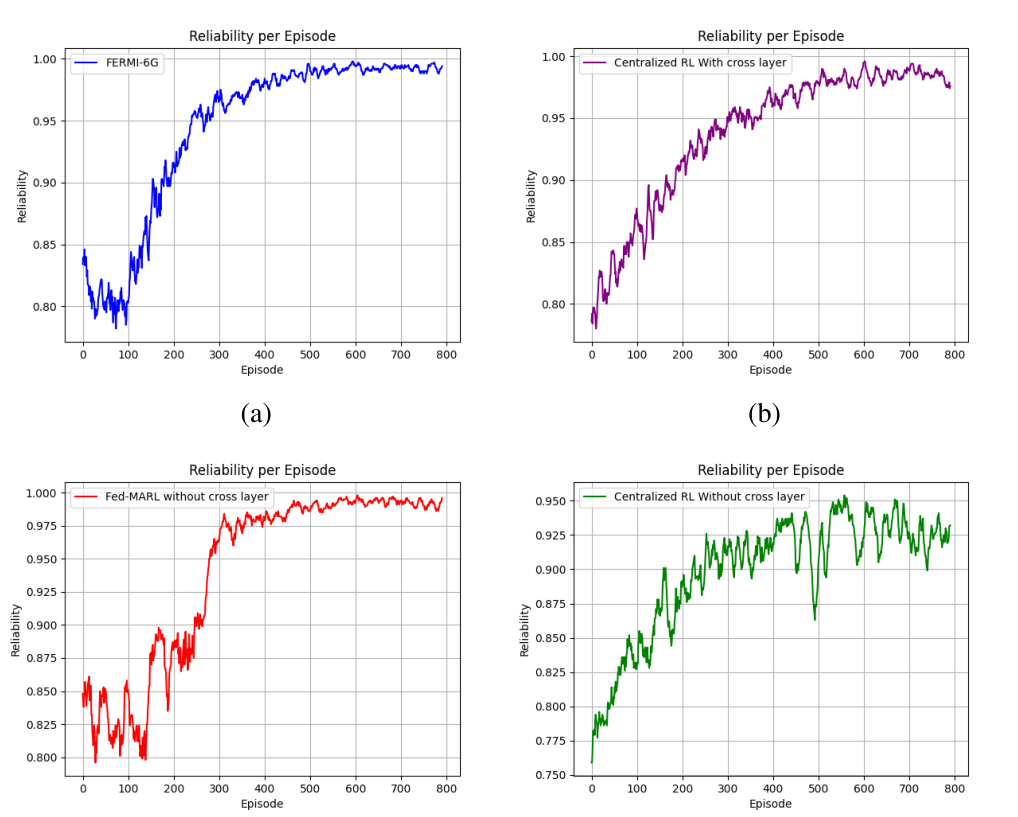
\includegraphics[width=0.64\textwidth]{figs/p2_reliability.png}
\caption{Reliability per episode: (a) FERMI-6G, (b) centralised RL with cross-layer optimisation, (c) Fed-MARL without cross-layer optimisation, (d) centralised RL \cite{p2}}
\label{fig:p2_rel}
\end{figure}

\paragraph{} \textbf{Scalability.} With 50 agents, FERMI-6G retains 90.01\% reliability and Fed-MARL 84.05\%, whereas the centralised frameworks collapse to 12.38\% and 20.69\% (Figure~\ref{fig:p2_chart}). The centralised cross-layer framework does achieve the lowest latency (0.92 s) and completion time, but in its simplified environment \cite{p2}.

\begin{figure}[htbp]
\centering
\begin{subfigure}[t]{0.49\textwidth}\centering
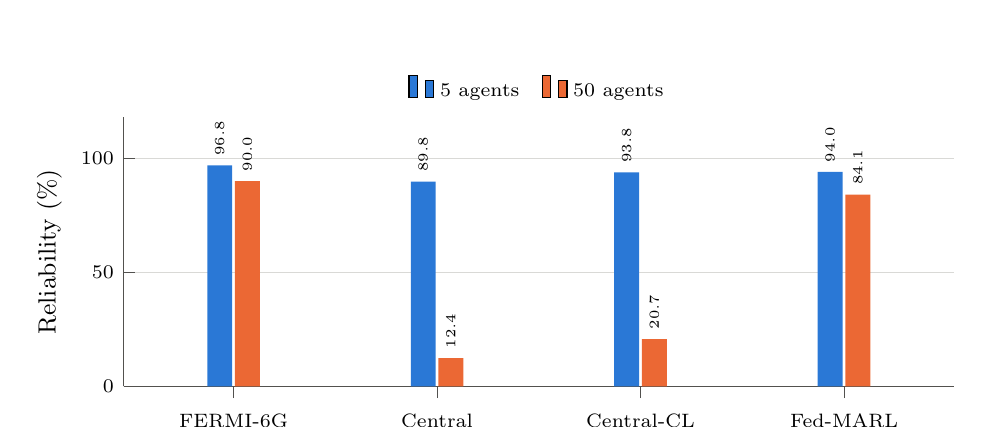
\begin{tikzpicture}
\begin{axis}[
  ybar=1pt, bar width=9pt, width=\linewidth, height=5.0cm,
  symbolic x coords={FERMI-6G,Central,Central-CL,Fed-MARL},
  xtick=data, enlarge x limits=0.18, ymin=0, ymax=118,
  ylabel={Reliability (\%)}, ylabel style={font=\small},
  ymajorgrids, grid style={gridgray}, axis line style={inkgray}, tick style={inkgray},
  axis x line*=bottom, axis y line*=left, tick label style={font=\scriptsize},
  nodes near coords, nodes near coords style={font=\tiny, text=black, rotate=90, anchor=west},
  every node near coord/.append style={/pgf/number format/fixed, /pgf/number format/fixed zerofill, /pgf/number format/precision=1},
  legend style={at={(0.5,1.02)}, anchor=south, legend columns=-1, draw=none, font=\scriptsize, /tikz/every even column/.append style={column sep=6pt}},
]
\addplot[fill=seriesA, draw=none] coordinates {(FERMI-6G,96.83) (Central,89.78) (Central-CL,93.81) (Fed-MARL,94.00)};
\addplot[fill=seriesB, draw=none] coordinates {(FERMI-6G,90.01) (Central,12.38) (Central-CL,20.69) (Fed-MARL,84.05)};
\legend{5 agents, 50 agents}
\end{axis}
\end{tikzpicture}
\caption{Reliability with 5 and 50 agents}
\end{subfigure}\hfill
\begin{subfigure}[t]{0.49\textwidth}\centering
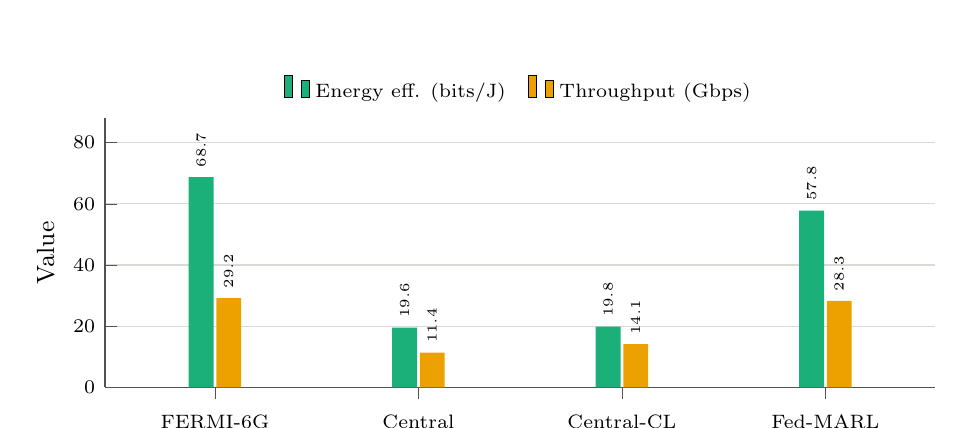
\begin{tikzpicture}
\begin{axis}[
  ybar=1pt, bar width=9pt, width=\linewidth, height=5.0cm,
  symbolic x coords={FERMI-6G,Central,Central-CL,Fed-MARL},
  xtick=data, enlarge x limits=0.18, ymin=0, ymax=88,
  ylabel={Value}, ylabel style={font=\small},
  ymajorgrids, grid style={gridgray}, axis line style={inkgray}, tick style={inkgray},
  axis x line*=bottom, axis y line*=left, tick label style={font=\scriptsize},
  nodes near coords, nodes near coords style={font=\tiny, text=black, rotate=90, anchor=west},
  every node near coord/.append style={/pgf/number format/fixed, /pgf/number format/fixed zerofill, /pgf/number format/precision=1},
  legend style={at={(0.5,1.02)}, anchor=south, legend columns=-1, draw=none, font=\scriptsize, /tikz/every even column/.append style={column sep=6pt}},
]
\addplot[fill=seriesC, draw=none] coordinates {(FERMI-6G,68.72) (Central,19.55) (Central-CL,19.84) (Fed-MARL,57.80)};
\addplot[fill=seriesD, draw=none] coordinates {(FERMI-6G,29.20) (Central,11.35) (Central-CL,14.11) (Fed-MARL,28.26)};
\legend{Energy eff. (bits/J), Throughput (Gbps)}
\end{axis}
\end{tikzpicture}
\caption{Energy efficiency and throughput}
\end{subfigure}
\caption{Scalability, energy efficiency, and throughput of the four frameworks, plotted from Table~\ref{tab:p2_results} (Central-CL: centralised RL with cross-layer optimisation)}
\label{fig:p2_chart}
\end{figure}

\subsection{Discussion}

\paragraph{} FERMI-6G shows that decentralised agents can learn a genuinely cross-layer policy while protecting their updates cryptographically, and that this scales far better than centralised control. The authors report its trade-offs candidly. Performance gains make agents more ``selfish'': their discussion notes fairness falling to about 0.37 against about 0.80 for the centralised cross-layer framework (Table~\ref{tab:p2_results} reports 0.79 and 0.99). Offloading delay (3.95 s) is high and spectral efficiency (about 0.20 bps/Hz) is far below 6G targets of 10--20 bps/Hz. The baselines ran in simplified environments, so numerical comparisons partly reflect environment differences; the main experiment uses only five agents; synchronisation every $K$ episodes is assumed; and the threat model covers only semi-honest adversaries, so poisoned updates from malicious agents would go undetected. Fed-MARL with heuristic MAC and CPU control is simpler and easier to tune, but in dynamic, congested networks FERMI-6G's learned cross-layer policy performs better.

% ---------------------------------------------------------------
\section{Federated Multi-Agent Deep Learning and Neural Networks for Advanced Distributed Sensing in Wireless Networks}

\paragraph{} Muller, DeRosa, Zhang, and Huan \cite{p3}, from the University of Oulu, survey multi-agent deep learning (MADL)---multi-agent DRL, federated training, and graph neural networks---for wireless systems in which sensing, communication, and computing are tightly coupled, with emphasis on 2021--2025 research. It is the broadest of the four works and the main source in this seminar for the network-security and UAV aspects of federated multi-agent AI.

\subsection{Scope, Background, and Reference Architecture}

\paragraph{} Integrated sensing and communication (ISAC), edge intelligence, open programmable RAN (O-RAN), and UAV networking create control problems that are decentralised, partially observed, time-varying, and resource-constrained \cite{p3}. The survey contributes a systems-to-algorithms \textbf{taxonomy}, a synthesis of \textbf{advanced techniques} (hierarchical and over-the-air FL, communication-efficient federated deep RL, serverless edge computing), coverage of \textbf{applications} (MEC offloading and slicing, UAV networks with power-domain NOMA, intrusion detection, ISAC), and an \textbf{open-issues agenda}. It models wireless problems as Markov games or Dec-POMDPs trained with CTDE, uses graph neural networks to exploit the permutation symmetry of interference graphs, and places learning agents at edge nodes that must act in real time. Figure~\ref{fig:p3_arch} redraws its three-plane reference architecture.

\begin{figure}[htbp]
\centering
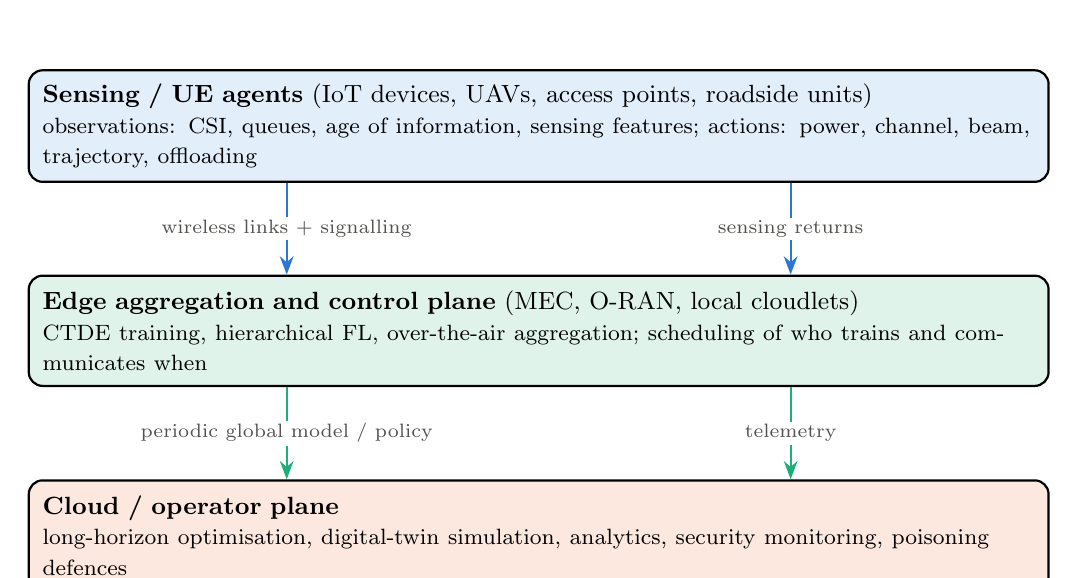
\begin{tikzpicture}[>=Stealth, thick,
  plane/.style={draw, rounded corners=5pt, text width=12.6cm, minimum height=1.4cm, font=\small, align=left, inner sep=5pt},
  lab/.style={font=\scriptsize, text=inkgray, fill=white, inner sep=1pt}]
\node[plane, fill=boxblue]   (u) at (0,0)    {\textbf{Sensing / UE agents} (IoT devices, UAVs, access points, roadside units)\\
  \footnotesize observations: CSI, queues, age of information, sensing features; actions: power, channel, beam, trajectory, offloading};
\node[plane, fill=boxgreen]  (e) at (0,-2.6) {\textbf{Edge aggregation and control plane} (MEC, O-RAN, local cloudlets)\\
  \footnotesize CTDE training, hierarchical FL, over-the-air aggregation; scheduling of who trains and communicates when};
\node[plane, fill=boxorange] (c) at (0,-5.2) {\textbf{Cloud / operator plane}\\
  \footnotesize long-horizon optimisation, digital-twin simulation, analytics, security monitoring, poisoning defences};
\draw[->, seriesA] ([xshift=-3.2cm]u.south) -- node[lab]{wireless links + signalling} ([xshift=-3.2cm]e.north);
\draw[->, seriesA] ([xshift=3.2cm]u.south) -- node[lab]{sensing returns} ([xshift=3.2cm]e.north);
\draw[->, seriesC] ([xshift=-3.2cm]e.south) -- node[lab]{periodic global model / policy} ([xshift=-3.2cm]c.north);
\draw[->, seriesC] ([xshift=3.2cm]e.south) -- node[lab]{telemetry} ([xshift=3.2cm]c.north);
\end{tikzpicture}
\caption{Conceptual architecture for distributed sensing, wireless communication, and multi-agent deep learning (redrawn from \cite{p3})}
\label{fig:p3_arch}
\end{figure}

\subsection{Advanced Techniques}

\paragraph{} \textbf{Multi-agent DRL} casts each base station, user, UAV, or slice controller as an agent, with \textbf{mean-field} approximations for dense networks and \textbf{constrained} formulations where QoS is non-negotiable. \textbf{GNN-based learning-to-optimise} generalises across network sizes through permutation equivariance. \textbf{Wireless FL} must be co-designed with client selection and power and bandwidth allocation; hierarchical FL reduces latency, and over-the-air aggregation trades speed for fading-induced error. \textbf{Federated deep RL} has been applied to cooperative edge caching and aerial relays---the vehicular and 6G frameworks of \cite{p1,p2} belong here. \textbf{Serverless edge computing} can package inference, aggregation, and monitoring as on-demand functions, at the risk of cold starts \cite{p3}. Table~\ref{tab:p3_paradigms} summarises the survey's comparison.

{\renewcommand{\arraystretch}{1.15}
\begin{table}[htbp]
\centering
\caption{Core learning paradigms and their suitability for wireless systems (adapted from \cite{p3})}\label{tab:p3_paradigms}
\small
\begin{tabularx}{\textwidth}{|p{2.6cm}|X|X|}
\hline
\textbf{Paradigm} & \textbf{Key strength} & \textbf{Key limitation} \\ \hline
CTDE MADRL & Captures coupling such as interference with low run-time signalling & Non-stationarity; scaling; safety and QoS constraints \\ \hline
Mean-field MADRL & Scales to dense deployments & May miss rare but critical interactions \\ \hline
GNN learning-to-optimise & Permutation equivariance; generalises across topologies & Graph and feature design; missing CSI \\ \hline
Wireless / hierarchical FL & Privacy by design; lower-latency aggregation & Communication bottleneck; heterogeneity; security threats \\ \hline
Federated deep RL & Distributed adaptation without sharing trajectories & Instability; partial observability; poisoning risks \\ \hline
Serverless orchestration & Elasticity; fits intermittent learning tasks & Cold starts; orchestration complexity \\ \hline
\end{tabularx}
\end{table}}

\subsection{Applications: UAV Networks, Sensing, and Security}

\paragraph{} For \textbf{MEC and slicing}, the survey cites slicing-aware offloading with an adaptive TD3 agent and constrained multi-agent RL for RAN slicing in O-RAN. For \textbf{UAV networks}, multi-agent DRL has optimised UAV \textbf{trajectories} for differentiated services, and \textbf{federated multi-agent DRL} has achieved fair communication and trajectory control across multiple UAVs while keeping each UAV's experience local; other work combines serverless FL with power-domain NOMA in UAV-enabled heterogeneous networks, and federated DRL jointly optimises UAV trajectory and beamforming in space--aerial--terrestrial relay networks with RIS and RSMA \cite{p3}. For \textbf{ISAC}, agents allocate beams and waveforms between sensing and communication and fuse detections across nodes for tracking. For \textbf{security}, intrusion detection in sensor networks increasingly uses FL for privacy and cross-domain training, but collaboratively trained detectors are exposed to \textbf{poisoning and backdoor} attacks, bridging ``sensing security'' and ``learning security'' \cite{p3}.

\subsection{Challenges and Future Directions}

\paragraph{} The survey identifies six challenges: \textbf{scalability and non-stationarity} in dense networks and swarms; \textbf{communication overhead}, since model updates compete with user traffic; \textbf{real-time safety}, where formal guarantees for deep RL are lacking; \textbf{adversarial security}, including poisoning, backdoors, observation spoofing, reward manipulation, and Byzantine agents; \textbf{heterogeneity and reproducibility}, given custom simulators and proprietary traces; and \textbf{operational complexity} of O-RAN control loops and serverless deployment. It proposes sense--communicate--compute co-design with hybrid model-based and learned controllers, constraint-aware and verifiable policies, graph-native multi-agent learning, federated RL at scale with robust aggregation, serverless learning control planes, and privacy-aware real-time ISAC intelligence \cite{p3}.

\subsection{Discussion}

\paragraph{} The survey connects the other works to a larger map---\cite{p1,p2} are federated deep RL for MEC, FERMI-6G's secure aggregation addresses one of its security concerns, and ComDML \cite{p4} answers its call for communication-efficient serverless learning---and it is the only work here to cover UAV trajectory control, intrusion detection, and ISAC. As a short survey, however, it contains no experiments, its comparisons are qualitative, and some in-text citation numbers do not match its reference list (for example, a citation for GNN-based radio resource management points to an unrelated routing paper), so original sources should be consulted directly.

% ---------------------------------------------------------------
\section{Communication-Efficient Training Workload Balancing for Decentralized Multi-Agent Learning}

\paragraph{} Mohammadabadi, Yang, Yan, and Zhang \cite{p4} propose \textbf{ComDML}, a decentralised multi-agent learning (DML) framework that balances training workload among heterogeneous agents without any central server: slow agents offload part of their model to fast agents using local-loss-based split training, and a decentralised scheduler decides the pairings.

\subsection{Problem Statement and Motivation}

\paragraph{} Devices differ in computation, bandwidth, and data size, so in synchronous training fast agents wait for \textbf{stragglers} and their spare capacity is wasted \cite{p4}. Split learning reduces device computation but waits for server gradients at every step; fixed-split and tier-based methods cannot adapt or still train the whole model on each device; and all of these need a server, which is a bottleneck and a target. Serverless methods such as gossip learning and BrainTorrent remove the server but ignore heterogeneity. ComDML minimises total training time in a heterogeneous, fully decentralised system.

\subsection{Local-Loss Split Training and Optimisation}

\paragraph{} The $K$ agents minimise the global objective of Equation~\ref{eq:flobj}. The model is split at one of $M$ points $m$ into a \textbf{slow agent-side} part $w^{a_m}_{s_i}$ and a \textbf{fast agent-side} part $w^{a_m}_{f_i}$. The slow agent trains its part with a small auxiliary network (a fully connected and an average-pooling layer) that provides a local loss, while the paired fast agent trains the remaining layers on the slow agent's intermediate outputs $z_n$---in parallel with its own training:
\begin{equation}
\min_{w^{a_m}_{s_i},\,w^{\mathrm{aux}_m}_i}\ \frac{1}{N_i}\sum_{n=1}^{N_i}\ell\big((x_n,y_n);(w^{a_m}_{s_i},w^{\mathrm{aux}_m}_i)\big),\qquad
\min_{w^{a_m}_{f_i}}\ \frac{1}{N_i}\sum_{n=1}^{N_i}\ell\big((z_n,y_n);w^{a_m}_{f_i}\big).
\end{equation}
Figure~\ref{fig:p4_balance} shows how offloading fills the fast agent's idle time \cite{p4}.

\begin{figure}[htbp]
\centering
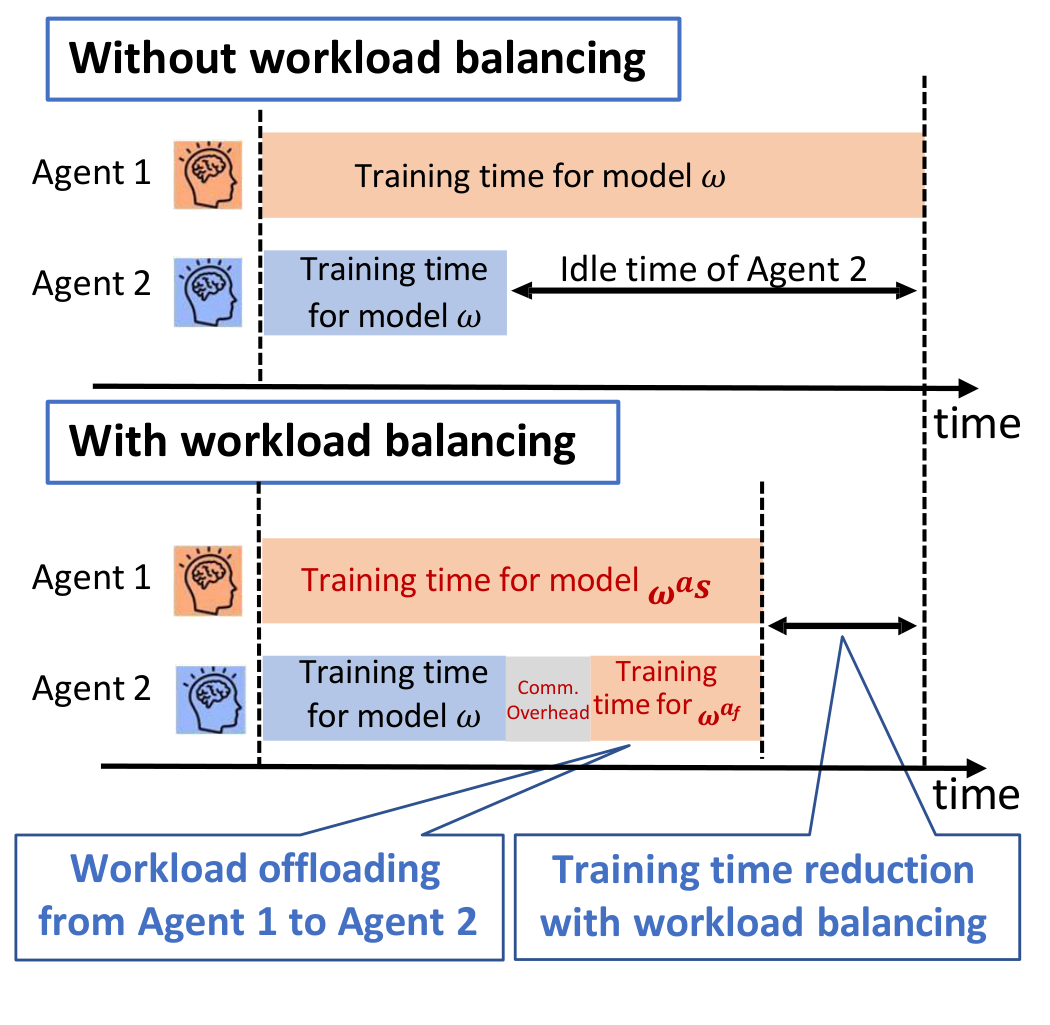
\includegraphics[width=0.46\textwidth]{figs/p4_fig1_balancing.png}
\caption{Training with and without workload balancing: offloading part of Agent 1's model to Agent 2 fills Agent 2's idle time and shortens the round \cite{p4}}
\label{fig:p4_balance}
\end{figure}

\paragraph{} With $\gamma_{ij}\in\{0,1\}$ indicating that agent $i$ offloads to agent $j$, an agent that does not offload spends its own computation time $\tau_i(w)$ plus the computation and communication for work accepted from slower agents, while an agent that offloads spends $\tau_i(w^{a_m}_{s_i})$ plus the communication time $\tau_{ij}$ of its intermediate data. Since the round ends when the slowest agent finishes, ComDML solves
\begin{equation}
\min_{\{\gamma_{ij}\},\{w^{a_m}_{f_i}\}}\ \max_i\ \tau_i\qquad\text{s.t.}\ \gamma_{ij}\in\{0,1\}\ \ \forall i,j,
\label{eq:p4_minmax}
\end{equation}
an integer program that is hard to solve exactly without a central scheduler \cite{p4}.

\subsection{Decentralised Pairing and Training Workflow}

\paragraph{} Each agent first profiles every split $m$: the relative training time of the slow side $T^{a_m}_s$ and fast side $T^{a_m}_f$ and the intermediate data size $\nu_m$ per batch. Each round, agents broadcast their processing speed $p_j$ and individual training time $\hat{\tau}_j$ and pair greedily, slowest first. Agent $i$ with $\tilde{N}_i$ batches estimates its time when offloading to $j$ over a link of speed $c_{ij}$ as
\begin{equation}
\hat{\tau}^{m}_{ij}=\max\Big(\frac{\tilde{N}_i}{p^{m}_i},\ \hat{\tau}_j+\frac{\tilde{N}_i\,\nu_m}{c_{ij}}+\frac{\tilde{N}_i}{p^{m}_j}\Big),\qquad p^{m}_i=\frac{p_i}{T^{a_m}_s},\ p^{m}_j=\frac{p_j}{T^{a_m}_f},
\end{equation}
and chooses the partner and split that minimise it. Paired agents then train in parallel, and all models are averaged with recursive halving-and-doubling \textbf{AllReduce}, needing $2\log_2K$ steps and no coordinator (Algorithm~\ref{alg:p4}, Figure~\ref{fig:p4_flow}) \cite{p4}.

\begin{algorithm}[htbp]
\caption{ComDML: decentralised pairing and training (adapted from \cite{p4})}\label{alg:p4}
\begin{algorithmic}[1]
\Require rounds $R$; split profiles $(T^{a_m}_s,T^{a_m}_f,\nu_m)$; agents sorted by training time (list $\mathcal{L}$)
\For{round $r=0$ to $R-1$}
  \State Each agent broadcasts $p_j$ and $\hat{\tau}_j$ to connected agents
  \For{each unpaired agent $i$ in order $\mathcal{L}$ (slowest first)}
    \State Compute $\hat{\tau}^{m}_{ij}$ for every unpaired neighbour $j$ and split $m$
    \State $(j^{\star},m^{\star})\gets\arg\min_{j,m}\hat{\tau}^{m}_{ij}$; pair with $j^{\star}$ if faster than training alone
  \EndFor
  \State Pairs perform local-loss split training in parallel; unpaired agents train alone
  \State Aggregate all models with decentralised AllReduce
\EndFor
\end{algorithmic}
\end{algorithm}

\begin{figure}[htbp]
\centering
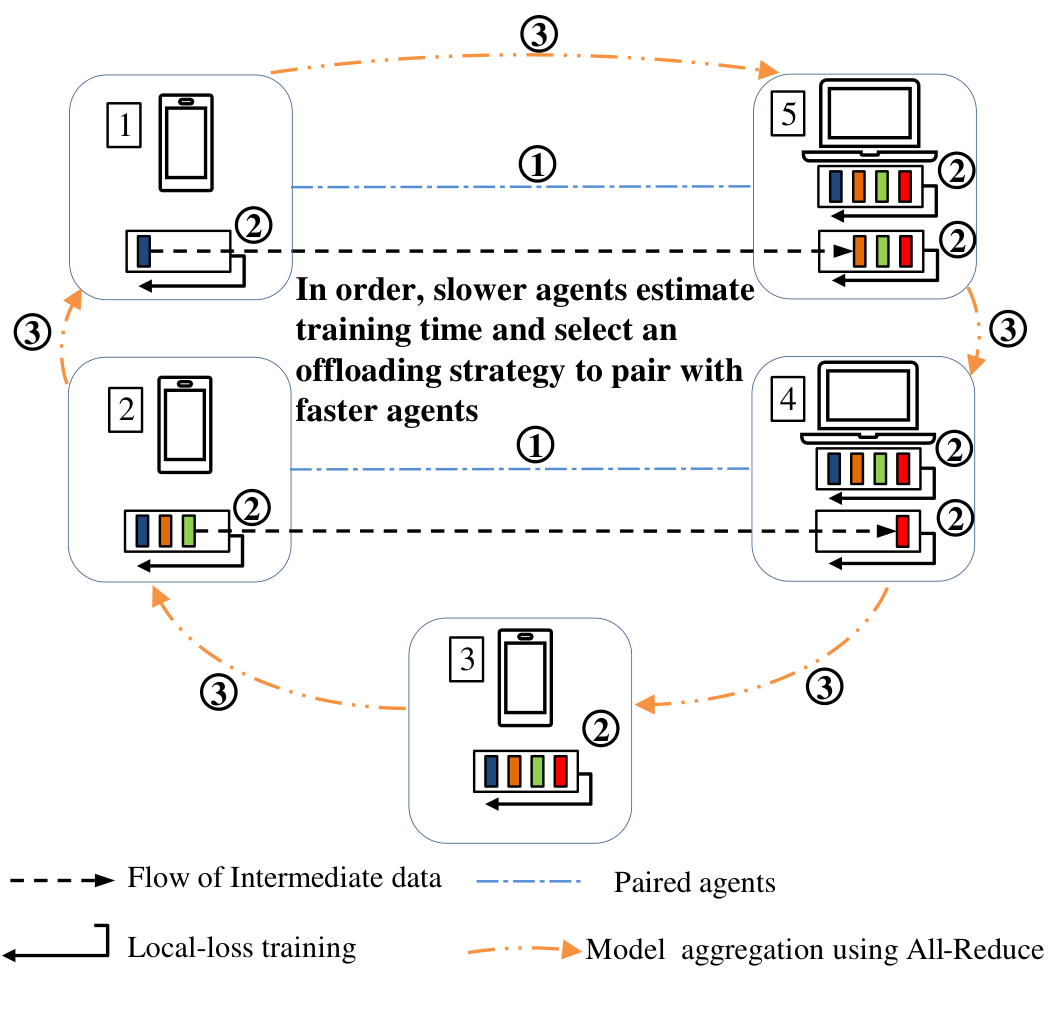
\includegraphics[width=0.44\textwidth]{figs/p4_fig2_workflow.png}
\caption{ComDML training round: agents 1 and 2 offload work to faster agents 5 and 4, agent 3 trains independently, and all models are aggregated with AllReduce \cite{p4}}
\label{fig:p4_flow}
\end{figure}

\paragraph{} \textbf{Privacy and convergence.} Fast agents' data are protected because communication is one-way, and slow agents can add PixelDP noise, patch shuffling, distance-correlation minimisation, or SplitGuard to their intermediate data, with DP or cryptography for aggregation. Under standard assumptions (smoothness, bounded gradients and variance, bounded dissimilarity), the slow-side model converges at rate $\mathcal{O}\big(\tfrac{1}{RA_m}+e^{-R}\big)$ for strongly convex losses and $\mathcal{O}\big(\tfrac{1}{\sqrt{RA_m}}+\tfrac{1}{R}\big)$ for non-convex ones, and the fast side converges at similar rates that depend on the slow side's convergence \cite{p4}.

\subsection{Experimental Setup}

\paragraph{} Experiments train ResNet-56 and ResNet-110 models on CIFAR-10, CIFAR-100, and CINIC-10, with non-IID variants from a Dirichlet distribution (concentration 0.5), against BrainTorrent, Gossip Learning, decentralised AllReduce, and FedAvg. Agents are given one of five CPU profiles (4 to 0.2 CPUs) and five link profiles (0 to 100 Mbps), and 20\% of profiles change every 100 rounds. Training uses SGD with momentum 0.9, learning rate 0.001, batch size 100, and one local epoch, in PyTorch on a server with four GTX 1080 Ti GPUs \cite{p4}.

\subsection{Results and Analysis}

\paragraph{} \textbf{Choosing the split.} Table~\ref{tab:p4_layers} shows two-agent training to 90\% accuracy. With 2 CPUs versus 0.25 CPU at 50 Mbps, offloading 37 layers cuts total time from 20{,}096 s to 9{,}352 s (\textbf{53\%}) by eliminating idle time; with 2 CPUs versus 1 CPU at 100 Mbps, the best choice is 19 layers and the gain is small. Offloading more layers lowers computation but can raise communication, so the best split depends on the resources---hence dynamic pairing \cite{p4}.

{\renewcommand{\arraystretch}{1.12}
\begin{table}[htbp]
\centering
\caption{Two-agent training time (s) to 90\% accuracy on CIFAR-10 with ResNet-56 for different numbers of offloaded layers \cite{p4}}\label{tab:p4_layers}
\small
\begin{tabular}{|c|c|c|c|c|c|c|c|c|}
\hline
\multirow{2}{*}{\textbf{Layers}} & \multicolumn{4}{c|}{\textbf{Setting 1: 2 vs 0.25 CPU, 50 Mbps}} & \multicolumn{4}{c|}{\textbf{Setting 2: 2 vs 1 CPU, 100 Mbps}} \\ \cline{2-9}
 & Train & Comm. & Idle & Total & Train & Comm. & Idle & Total \\ \hline
0 & 5573 & 34 & 14489 & 20096 & 5578 & 17 & 3560 & 9165 \\ \hline
10 & 6740 & 3532 & 4787 & 15059 & 6364 & 1766 & 350 & 8481 \\ \hline
19 & 7625 & 3544 & 1682 & 12851 & 6547 & 1772 & 137 & \textbf{8456} \\ \hline
28 & 7906 & 1261 & 2049 & 11217 & 7859 & 630 & 3368 & 8490 \\ \hline
37 & 8003 & 1265 & 84 & \textbf{9352} & 8275 & 632 & 7318 & 8908 \\ \hline
55 & 10343 & 640 & 9833 & 10983 & 10101 & 320 & 9964 & 10421 \\ \hline
\end{tabular}
\end{table}}

\paragraph{} \textbf{Comparison with baselines.} With 10 heterogeneous agents, ComDML is fastest on every dataset in both IID and non-IID settings (Table~\ref{tab:p4_time}, Figure~\ref{fig:p4_chart}). On IID CIFAR-10 it needs 7{,}211 s against 24{,}174 s for FedAvg and 24{,}639 s for BrainTorrent---\textbf{70\%} and \textbf{71\%} less---at the same target accuracy \cite{p4}.

{\renewcommand{\arraystretch}{1.12}
\begin{table}[htbp]
\centering
\caption{Training time (s) with 10 agents to reach the target accuracy (CIFAR-10: 90\% IID / 85\% non-IID; CIFAR-100: 65\% / 60\%; CINIC-10: 75\% / 65\%) \cite{p4}}\label{tab:p4_time}
\small
\begin{tabular}{|l|c|c|c|c|c|c|}
\hline
\multirow{2}{*}{\textbf{Method}} & \multicolumn{2}{c|}{\textbf{CIFAR-10}} & \multicolumn{2}{c|}{\textbf{CIFAR-100}} & \multicolumn{2}{c|}{\textbf{CINIC-10}} \\ \cline{2-7}
 & IID & non-IID & IID & non-IID & IID & non-IID \\ \hline
\textbf{ComDML} & \textbf{7211} & \textbf{4177} & \textbf{5589} & \textbf{8104} & \textbf{10229} & \textbf{17208} \\ \hline
Gossip Learning & 20337 & 15269 & 15262 & 28621 & 24636 & 56325 \\ \hline
BrainTorrent & 24639 & 14323 & 18046 & 25867 & 31992 & 51144 \\ \hline
AllReduce & 25153 & 13859 & 18462 & 26623 & 32652 & 53265 \\ \hline
FedAvg & 24174 & 13095 & 17630 & 25113 & 30601 & 49624 \\ \hline
\end{tabular}
\end{table}}

\begin{figure}[htbp]
\centering
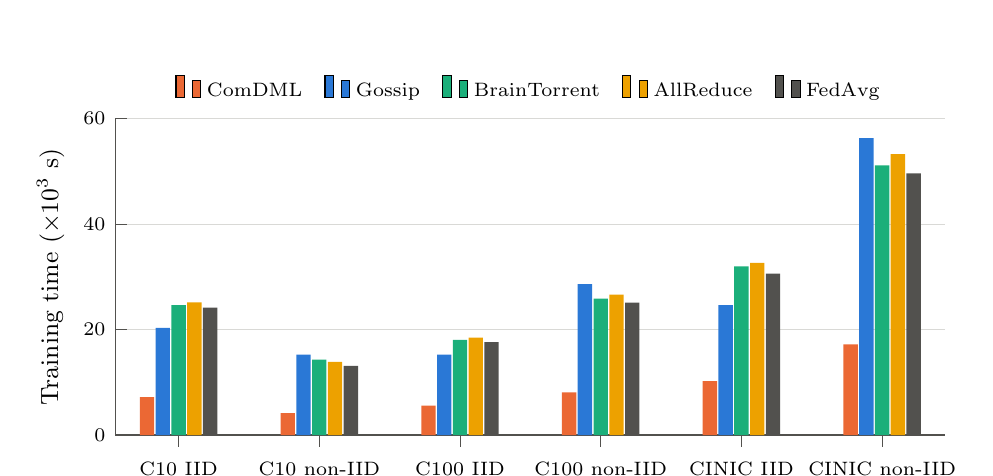
\begin{tikzpicture}
\begin{axis}[
  ybar=0.5pt, bar width=5.2pt, width=\textwidth, height=5.6cm,
  symbolic x coords={C10 IID,C10 non-IID,C100 IID,C100 non-IID,CINIC IID,CINIC non-IID},
  xtick=data, enlarge x limits=0.09, ymin=0, ymax=60,
  ylabel={Training time ($\times10^{3}$ s)}, ylabel style={font=\small},
  ymajorgrids, grid style={gridgray}, axis line style={inkgray}, tick style={inkgray},
  axis x line*=bottom, axis y line*=left, tick label style={font=\scriptsize},
  legend style={at={(0.5,1.02)}, anchor=south, legend columns=-1, draw=none, font=\scriptsize, /tikz/every even column/.append style={column sep=6pt}},
]
\addplot[fill=seriesB, draw=none] coordinates {(C10 IID,7.211) (C10 non-IID,4.177) (C100 IID,5.589) (C100 non-IID,8.104) (CINIC IID,10.229) (CINIC non-IID,17.208)};
\addplot[fill=seriesA, draw=none] coordinates {(C10 IID,20.337) (C10 non-IID,15.269) (C100 IID,15.262) (C100 non-IID,28.621) (CINIC IID,24.636) (CINIC non-IID,56.325)};
\addplot[fill=seriesC, draw=none] coordinates {(C10 IID,24.639) (C10 non-IID,14.323) (C100 IID,18.046) (C100 non-IID,25.867) (CINIC IID,31.992) (CINIC non-IID,51.144)};
\addplot[fill=seriesD, draw=none] coordinates {(C10 IID,25.153) (C10 non-IID,13.859) (C100 IID,18.462) (C100 non-IID,26.623) (CINIC IID,32.652) (CINIC non-IID,53.265)};
\addplot[fill=inkgray, draw=none] coordinates {(C10 IID,24.174) (C10 non-IID,13.095) (C100 IID,17.630) (C100 non-IID,25.113) (CINIC IID,30.601) (CINIC non-IID,49.624)};
\legend{ComDML, Gossip, BrainTorrent, AllReduce, FedAvg}
\end{axis}
\end{tikzpicture}
\caption{Training time to target accuracy with 10 heterogeneous agents, plotted from Table~\ref{tab:p4_time}}
\label{fig:p4_chart}
\end{figure}

\paragraph{} \textbf{Scalability, privacy, and topology.} Training to 80\% accuracy on IID CIFAR-10 with 20, 50, and 100 agents, ComDML stays fastest for both models; with 100 agents and ResNet-110 it needs 15{,}843 s against 29{,}494 s for FedAvg and 31{,}526 s for BrainTorrent. With 100 agents it reaches 81.7\% accuracy with distance correlation, 83.2\% with patch shuffling, and 77.6\% with Laplace DP ($\epsilon=0.5$), and it remains fastest when only 20\% of links are available, because it adapts its pairings and lets poorly connected agents train alone \cite{p4}.

\subsection{Discussion}

\paragraph{} ComDML's insight is that heterogeneity is an opportunity: fast agents' idle capacity can absorb slow agents' work, provided the communication cost of the split is counted. Its pairing needs only lightweight profiling and neighbour information, it scales to 100 agents with up to 71\% shorter training, and it offers convergence guarantees for split models. Its limitations are that heterogeneity is simulated on one server, the experiments cover image classification rather than multi-agent control, the greedy pairing is heuristic with one partner per slow agent, and malicious agents are not considered.

% ---------------------------------------------------------------
\section{Summary of the Reviewed Papers}

\paragraph{} Table~\ref{tab:summary} summarises the four works; the next chapter compares them in detail.

{\renewcommand{\arraystretch}{1.15}
\begin{table}[htbp]
\centering
\caption{Summary of the reviewed works}\label{tab:summary}
\small
\begin{tabularx}{\textwidth}{|p{2.25cm}|p{2.6cm}|X|X|}
\hline
\textbf{Work} & \textbf{Problem} & \textbf{Technique} & \textbf{Headline result} \\ \hline
Shabir et al. \cite{p1} & Offloading in vehicular fog computing & Multi-agent A3C with two-tier vehicle--fog federation & 58.6\% lower residence time and 57.11\% lower delay at $\lambda=200$ \\ \hline
Andong and Min \cite{p2} & Cross-layer 6G edge resource management & DRQN agents, cross-layer actions, ECDH/AES secure aggregation & 96.83\% reliability; 0.023 J/task; 90\% reliability with 50 agents \\ \hline
Muller et al. \cite{p3} & Federated MADL for wireless sensing & Survey of MADRL, FL/FRL, GNNs, serverless orchestration & Agenda: scalability, security, real-time safety \\ \hline
Mohammad\-abadi et al. \cite{p4} & Stragglers in serverless training & Local-loss split training, greedy pairing, AllReduce & Up to 71\% shorter training at equal accuracy \\ \hline
\end{tabularx}
\end{table}}

% ================= CHAPTER 4: DISCUSSION & COMPARISON =================
\chapter{Discussion \& Comparison}

\paragraph{} This chapter compares the four reviewed works. All concern learning across many agents without centralising their data, but they target different problems and evaluate in different environments. The comparison highlights their complementary strengths and the trade-offs among learning speed, communication, security, fairness, and deployability.

\section{Analytical Focus and Methodology}

\paragraph{} The works examine federated multi-agent learning from four angles: the \textbf{decision problem} of where vehicles should offload tasks \cite{p1}; \textbf{joint cross-layer control with private model exchange} in 6G \cite{p2}; the \textbf{landscape} of formulations, architectures, and applications, including security and UAV networks \cite{p3}; and the \textbf{training process itself} for heterogeneous agents without a server \cite{p4}. Together they span the stack from application-level decisions to the mechanics of distributed training. Table~\ref{tab:cmp_method} compares their methodologies.

{\renewcommand{\arraystretch}{1.15}
\begin{table}[htbp]
\centering
\caption{Methodological comparison of the reviewed works}\label{tab:cmp_method}
\small
\begin{tabularx}{\textwidth}{|p{2.2cm}|X|X|X|X|}
\hline
\textbf{Aspect} & \textbf{Shabir et al. \cite{p1}} & \textbf{Andong \& Min \cite{p2}} & \textbf{Muller et al. \cite{p3}} & \textbf{Mohammad\-abadi et al. \cite{p4}} \\ \hline
Agents & Moving vehicles & 6G edge devices & UEs, APs, UAVs, sensors & Heterogeneous devices \\ \hline
Learning task & Offloading policy (RL) & Cross-layer policy (RL) & RL, supervised, GNN & Image classification \\ \hline
Formulation & Per-agent MDP, residence-time reward & POMMDP, multi-objective reward & Markov games, Dec-POMDP, CTDE & Min--max training time \\ \hline
Agent model & A3C actor-critic & DRQN with LSTM & DRL, GNN, attention & Split ResNet + auxiliary net \\ \hline
Coordination & Vehicles $\rightarrow$ fog federation, asynchronous & Secure aggregation every $K$ episodes & Client--server, hierarchical, OTA, serverless & Serverless AllReduce with pairing \\ \hline
Privacy & Data local; plain updates & ECDH + AES masking & Surveys poisoning and defences & Split-data protection; optional DP \\ \hline
Evaluation & SUMO, $\lambda=60$--$200$ & 6G simulator, 800 episodes & Qualitative & CIFAR, CINIC; up to 100 agents \\ \hline
\end{tabularx}
\end{table}}

\section{Agent Design and Coordination Structure}

\paragraph{} The two RL papers design their agents differently. Paper \cite{p1} uses an \textbf{actor-critic} trained online with A3C: parallel environments decorrelate updates, no replay is needed, and the small action space (four destinations) suits a fast-changing environment. Paper \cite{p2} uses a \textbf{value-based} DRQN whose LSTM memory addresses partial observability explicitly, with prioritised replay and a richer composite action and multi-objective reward that reflect 6G's demands. The survey \cite{p3} points to further options---GNNs, attention, mean-field agents---that neither uses, and ComDML \cite{p4} decides where to \emph{split} a model between devices, an idea that could help the RL papers train larger policies on weak hardware.

\paragraph{} Coordination determines who talks to whom and whom everyone must trust. In \cite{p1} it is \textbf{hierarchical and asynchronous}, suited to intermittent vehicular connectivity; in \cite{p2} it is \textbf{synchronous and periodic}, with a server that sees only masked updates; in \cite{p4} it is \textbf{fully serverless}, removing the single point of failure and trust. Figure~\ref{fig:designspace} places the systems on two axes: decentralisation of training and protection of individual updates. No reviewed system reaches the upper-right region---decentralised, cryptographically private, \emph{and} robust to malicious agents---which is where future FedMARL systems should aim.

\begin{figure}[htbp]
\centering
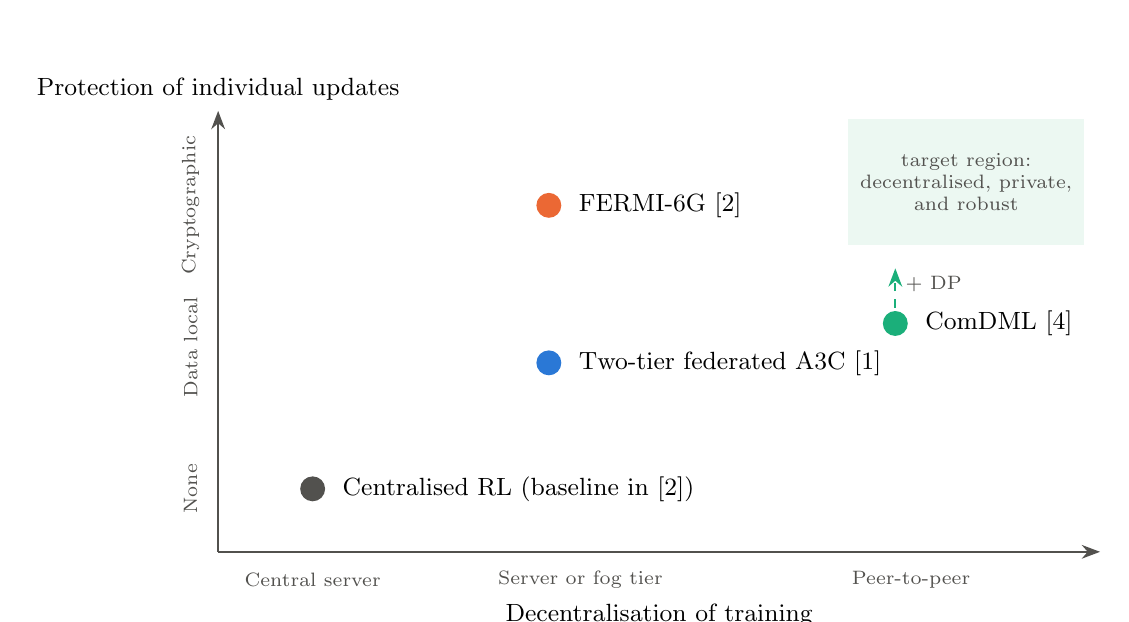
\begin{tikzpicture}[>=Stealth, thick,
  pt/.style={circle, fill=#1, minimum size=9pt, inner sep=0pt},
  lab/.style={font=\small, align=left, anchor=west}]
\draw[->, inkgray] (0,0) -- (11.2,0);
\node[font=\small] at (5.6,-0.8) {Decentralisation of training};
\draw[->, inkgray] (0,0) -- (0,5.6) node[above, font=\small, text=black]{Protection of individual updates};
\foreach \x/\t in {1.2/Central server,4.6/Server or fog tier,8.8/Peer-to-peer} \node[font=\scriptsize, text=inkgray] at (\x,-0.35) {\t};
\foreach \y/\t in {0.8/None,2.6/Data local,4.4/Cryptographic} \node[font=\scriptsize, text=inkgray, rotate=90] at (-0.35,\y) {\t};
\fill[boxgreen, opacity=0.6] (8.0,3.9) rectangle (11.0,5.5);
\node[font=\scriptsize, align=center, text=inkgray] at (9.5,4.7) {target region:\\ decentralised, private,\\ and robust};
\node[pt=inkgray] at (1.2,0.8) {}; \node[lab] at (1.45,0.8) {Centralised RL (baseline in [2])};
\node[pt=seriesA] at (4.2,2.4) {}; \node[lab] at (4.45,2.4) {Two-tier federated A3C [1]};
\node[pt=seriesB] at (4.2,4.4) {}; \node[lab] at (4.45,4.4) {FERMI-6G [2]};
\node[pt=seriesC] at (8.6,2.9) {}; \node[lab] at (8.85,2.9) {ComDML [4]};
\draw[->, dashed, seriesC] (8.6,3.1) -- (8.6,3.6) node[right, font=\scriptsize, text=inkgray, pos=0.6]{+ DP};
\end{tikzpicture}
\caption{Qualitative design space of the reviewed systems: degree of decentralisation versus protection of individual model updates}
\label{fig:designspace}
\end{figure}

\section{Robustness to Heterogeneity}

\paragraph{} \textbf{Environmental heterogeneity} is handled in \cite{p1} by aggregating across parallel environments and in \cite{p2} by recurrent memory and adaptive reward weights. \textbf{Statistical heterogeneity} (non-IID data) is tested only in \cite{p4}, whose speed-up persists under Dirichlet-skewed labels. \textbf{System heterogeneity} is the core of \cite{p4}, which exploits it through workload offloading, and is handled in \cite{p2} by excluding low-energy agents from aggregation.

\section{Security and Privacy}

\paragraph{} Security differs most across the works (Table~\ref{tab:cmp_security}). All keep raw data local. Only \cite{p2} protects individual updates cryptographically, and only against semi-honest adversaries; \cite{p4} protects intermediate data and supports DP at a cost of a few accuracy points; \cite{p1} acknowledges that its plain updates are open to gradient spoofing; and only the survey \cite{p3} examines \textbf{malicious} participants---poisoning, backdoors, observation spoofing, and reward manipulation. The mechanisms can conflict: secure aggregation and DP hide exactly the evidence needed to detect poisoned updates. Aggregation that is both \emph{private} and \emph{robust}---trust-aware aggregation---is therefore essential in adversarial settings such as network security and contested UAV operations.

{\renewcommand{\arraystretch}{1.15}
\begin{table}[htbp]
\centering
\caption{Threats and protection mechanisms across the reviewed works}\label{tab:cmp_security}
\small
\begin{tabularx}{\textwidth}{|p{3.1cm}|X|X|X|X|}
\hline
\textbf{Threat} & \textbf{\cite{p1}} & \textbf{\cite{p2}} & \textbf{\cite{p3}} & \textbf{\cite{p4}} \\ \hline
Raw-data exposure & Protected & Protected & Discussed & Protected \\ \hline
Inference from updates & Not protected & ECDH + AES masking & Discussed & Optional DP, data shielding \\ \hline
Single point of failure & Fog server & Aggregation server & Discussed & Removed \\ \hline
Poisoning, backdoors & Not addressed & Not addressed & Surveyed & Not addressed \\ \hline
\end{tabularx}
\end{table}}

\section{Scalability, Communication, and Results}

\paragraph{} FERMI-6G keeps 90.01\% reliability with 50 agents while centralised RL collapses to 12.38\% \cite{p2}; ComDML keeps its advantage from 10 to 100 agents and on sparse topologies \cite{p4}; the vehicular framework has 100 vehicles, but its fog-tier scalability is argued rather than measured \cite{p1}. Communication is reduced by sharing parameters instead of state \cite{p1}, by aggregating only every $K$ episodes and letting low-energy agents skip rounds \cite{p2}, and by modelling communication time explicitly in pairing \cite{p4}; ComDML's split experiment shows that ignoring communication can cancel the benefit of offloading. The headline results---58.6\% lower residence time \cite{p1}, 96.83\% reliability at one-third of centralised energy \cite{p2}, and up to 71\% shorter training \cite{p4}---measure different quantities and are not directly comparable. They also come with costs: FERMI-6G has higher offloading delay, lower spectral efficiency, and lower fairness than the centralised cross-layer controller, and the vehicular scheme has higher transmission delay than greedy offloading.

\section{Real-World Deployability}

\paragraph{} All three technical works rely on simulation---SUMO mobility with a simplified channel \cite{p1}, a detailed but laptop-scale 6G simulator with five agents \cite{p2}, and simulated heterogeneity on a GPU server \cite{p4}---and none reports a hardware testbed. Deployment would also require tolerating dropped participants, authenticating devices, and integrating with network management such as O-RAN \cite{p3}.

\section{Overall Comparative Insights}

\paragraph{} A consistent pattern emerges. \textbf{First}, federating locally trained models rather than raw data lets agents learn faster and more robustly than independent learning, whether they are vehicles, 6G devices, or trainers of a shared model. \textbf{Second}, this costs coordination overhead and, where a server is used, a single point of trust. \textbf{Third}, domain-specific design---residence-time rewards, cross-layer actions, profiled model splits---captures each problem's structure. \textbf{Fourth}, security has mainly meant privacy against curious observers; robustness to malicious participants is largely unaddressed. Hybrid architectures with trust-aware aggregation are therefore the most promising path forward.

% ================= CHAPTER 5: APPLICATIONS =================
\chapter{Applications}

\paragraph{} Federated multi-agent learning is relevant wherever many autonomous entities must coordinate without sharing raw data. This chapter outlines the main applications and relates them to the reviewed works.

\section{Connected and Autonomous Vehicles}

\paragraph{} Vehicles generate delay-sensitive workloads such as perception, route planning, and cooperative driving, and vehicular fog computing lets them share idle resources. The base paper \cite{p1} shows that federated multi-agent DRL can decide where each task should run, sharply reducing residence time and failures under heavy load. The same approach extends to V2X channel and power selection, roadside caching, and platoon coordination. Federation matters because trajectories and requests are privacy-sensitive and no vehicle stays connected to one server for long.

\section{6G Edge Networks and Mobile Edge Computing}

\paragraph{} In ultra-dense 6G networks, devices must choose offloading, channels, and CPU speed under URLLC, eMBB, and mMTC requirements and limited batteries. FERMI-6G \cite{p2} shows that federated agents can learn these decisions jointly and scale to 50 agents with 90\% reliability while secure aggregation protects each device's model. Related applications include slicing-aware offloading, constrained multi-agent RAN slicing in O-RAN, and federated cooperative edge caching \cite{p3}.

\section{Network Security and Intrusion Detection}

\paragraph{} Intrusion detection in sensor and IoT networks needs models trained on confidential traffic spread across many nodes. Federated learning lets nodes collaboratively train detectors, including for unseen attacks, without revealing traffic, and multi-agent formulations let them coordinate responses such as isolating compromised nodes \cite{p3}. The learning process, however, becomes part of the attack surface: a few compromised nodes can poison the shared detector or implant a backdoor. Secure aggregation \cite{p2} and robust aggregation \cite{p3} are therefore directly relevant, and security is where trust-aware aggregation is most urgently needed.

\section{UAV Trajectory Planning and Aerial Networks}

\paragraph{} UAVs serve as flying base stations, relays, and data collectors, and their trajectories determine coverage, throughput, fairness, and energy use jointly with power, association, and multiple-access decisions. Federated multi-agent DRL lets a swarm learn fair communication and trajectory policies while each UAV keeps its own experience, and federated DRL has optimised trajectory and beamforming together in space--aerial--terrestrial relay networks \cite{p3}. Federation suits UAVs because their links are intermittent and bandwidth-limited, and ComDML-style balancing \cite{p4} could let small UAVs offload training to ground stations.

\section{Sensing, Smart Cities, and Collaborative Training}

\paragraph{} In ISAC and perceptive networks, agents allocate beams between sensing and communication and fuse detections for tracking, and federated training enables collaborative recognition without centralising raw sensing streams \cite{p3}. Similar patterns arise in smart cities, industrial IoT, swarm robotics, and healthcare. Finally, collaborative training is itself an application: ComDML \cite{p4} shows that heterogeneous participants can train ResNet-scale models up to 71\% faster without a server, a capability that RL agents will need as their models grow.

% ================= CHAPTER 6: CHALLENGES AND FUTURE DIRECTIONS =================
\chapter{Challenges and Future Directions}

\paragraph{} Despite the progress shown by the reviewed works, several obstacles remain before federated multi-agent learning becomes standard practice. This chapter summarises the challenges of each work and of the field, and outlines future directions.

\section{Challenges Identified in the Reviewed Works}

\paragraph{} \textbf{Shabir et al. \cite{p1}} compare only with heuristics, assume a homogeneous quasi-static channel, use two training threads, and exchange updates in plain form; the authors plan more sophisticated DRL, better sampling efficiency, and less gradient traffic. \textbf{Andong and Min \cite{p2}} trade fairness for performance, have high offloading delay and low spectral efficiency, use five agents and simplified baselines, and defend only against semi-honest adversaries; they plan wider channels, power control, massive MIMO, edge-native low-latency techniques, fairness-aware coordination, and testbed validation. \textbf{Mohammadabadi et al. \cite{p4}} simulate heterogeneity, study only image classification, use heuristic one-to-one pairing, and ignore malicious agents.

\section{Cross-Cutting Challenges}

\paragraph{} \textbf{Non-stationarity and partial observability}: each agent's environment shifts as others learn, and averaging policies from different local conditions can blur behaviour that should differ. \textbf{Cost of learning}: model exchange uses the very spectrum and energy the agents manage, so update frequency, size, and participation must be optimised with the task. \textbf{Security versus privacy}: hiding updates helps privacy but hinders poisoning detection. \textbf{Fairness}: maximising overall performance can make agents selfish, yet fair sharing of spectrum, servers, and UAV coverage is often a requirement. \textbf{Heterogeneity}: synchronous rounds waste fast agents' capacity, while asynchronous ones risk stale updates. \textbf{Simulation-to-reality gap}: results come from differing simulators, and standard open benchmarks are lacking \cite{p3}. \textbf{Safety}: URLLC control, driving, and UAV flight need guarantees that current deep RL policies cannot provide.

\section{Future Research Directions}

\paragraph{} \textbf{Trust-aware aggregation}, combining secure and robust aggregation through secure computation of robust statistics, reputation-weighted averaging, or verifiable training, is the most important gap identified here, especially for security and UAV applications. \textbf{Hybrid FedMARL architectures} can combine recurrent, cross-layer agents \cite{p2}, hierarchical asynchronous aggregation for mobility \cite{p1}, serverless workload-balanced training \cite{p4}, and graph-based or mean-field policies for scale \cite{p3}. \textbf{Communication- and energy-aware federation} can use compression, event-triggered aggregation, over-the-air computation, and battery-aware participation, treating learning as another resource to schedule. \textbf{Fairness-aware coordination} can add Jain's index or worst-agent constraints to shared rewards. \textbf{Digital twins and real testbeds} can supply CTDE training environments and validate simulated gains, and \textbf{safe, verifiable policies} with feasibility layers and robust training are needed for safety-critical use \cite{p3}.

\section{Ethical and Societal Considerations}

\paragraph{} Federated multi-agent AI can strengthen privacy by keeping data on devices, but updates can still leak information and distributed sensing can enable surveillance. Safety-relevant decisions---offloading for vehicles, UAV flight, intrusion response---must be tested for failure and manipulation, with clear responsibility. The energy cost of training and communication should also be counted.

\section{Summary}

\paragraph{} The main challenges are non-stationarity, the cost of learning, the privacy--robustness tension, fairness, heterogeneity, the simulation-to-reality gap, and safety; progress requires trust-aware aggregation, hybrid architectures, efficient federation, and real-world validation.

% ================= CHAPTER 7: CONCLUSION =================
\chapter{Conclusion}

\paragraph{} Multi-agent AI systems---connected vehicles, 6G edge devices, sensor networks, and UAV swarms---must learn to coordinate from decentralised experience without exposing raw, privacy-sensitive data. Federated learning makes this possible by sharing models instead of data, and FedMARL lets agents that each see only part of the world learn policies informed by the experience of all. This seminar reviewed four recent works that apply this idea to distinct coordination problems.

\paragraph{} \textbf{Paper \cite{p1}}, the base paper, proposed two-tier federated A3C learning for vehicular fog computing, reducing residence time by 58.6\% and end-to-end delay by 57.11\% at heavy load. \textbf{Paper \cite{p2}} introduced FERMI-6G, whose DRQN agents jointly decide offloading, channel, and CPU frequency and synchronise through ECDH-based secure aggregation, achieving 96.83\% reliability, the lowest energy per task, and 90\% reliability with 50 agents where centralised RL collapsed. \textbf{Paper \cite{p3}} surveyed federated multi-agent deep learning for wireless sensing, including UAV networks and intrusion detection, and set out open problems in scalability, security, and safety. \textbf{Paper \cite{p4}} presented ComDML, cutting serverless training time by up to 71\% by balancing workload between heterogeneous agents. The comparison leads to four conclusions:
\begin{itemize}
  \item \textbf{Federation accelerates multi-agent learning} across very different domains.
  \item \textbf{Coordination has a cost} in overhead and trust, which hierarchical, asynchronous, and serverless designs reduce in different ways.
  \item \textbf{Agent design must fit the domain}, through suitable rewards, actions, memory, and model splits.
  \item \textbf{Security must go beyond privacy}: robustness to poisoning, backdoors, and spoofing is the key open problem for network security and UAV applications.
\end{itemize}

\paragraph{} Comparing these systems across agent design, coordination structure, robustness to heterogeneity, and real-world deployability therefore reveals a consistent pattern: federating locally trained policies rather than raw data lets systems as different as connected vehicles, edge devices, sensor networks, and UAV swarms reach faster, more robust joint behaviour than independent learning---at the cost of coordination overhead and, where a server is used, a single point of trust. Hybrid FedMARL architectures, combining domain-specific agent design with trust-aware aggregation, are the most promising direction for scalable, privacy-preserving multi-agent AI.

\paragraph{} For practitioners designing such a system, the reviewed work suggests a practical recipe: formulate the problem as a partially observable multi-agent decision process with a reward that directly reflects the service objective, such as residence time or deadline-normalised latency; give each agent a recurrent or actor-critic model sized for its hardware; train locally and aggregate periodically through a hierarchy that matches the network, such as vehicles to fog servers or devices to edge servers; protect updates with secure aggregation and, where feasible, differential privacy; let low-energy or slow agents skip rounds or offload part of their training to faster peers; monitor fairness and robustness alongside performance; and validate in realistic simulators and testbeds before deployment. Following this recipe brings together the strengths of all four works and moves toward the goal expressed in the title of this seminar: federated learning that makes multi-agent AI faster, more private, and more trustworthy across vehicular communication, network security, and UAV trajectory planning.

% ================= REFERENCES =================
\begingroup
\setstretch{1.15}
\begin{thebibliography}{99}
\addcontentsline{toc}{chapter}{References}

\bibitem{p1}
B. Shabir, A. U. Rahman, A. W. Malik, R. Buyya, and M. A. Khan, ``A federated multi-agent deep reinforcement learning for vehicular fog computing,'' \textit{The Journal of Supercomputing}, Springer, 2022, doi: 10.1007/s11227-022-04911-8.

\bibitem{p2}
F. J. E. N. Andong and Q. Min, ``Federated multi-agent reinforcement learning for privacy-preserving and energy-aware resource management in 6G edge networks,'' arXiv preprint arXiv:2509.10163, Sep. 2025.

\bibitem{p3}
N. Muller, S. DeRosa, S. Zhang, and C. L. Huan, ``Federated multi-agent deep learning and neural networks for advanced distributed sensing in wireless networks,'' arXiv preprint arXiv:2603.16881, 2026.

\bibitem{p4}
S. M. S. Mohammadabadi, L. Yang, F. Yan, and J. Zhang, ``Communication-efficient training workload balancing for decentralized multi-agent learning,'' arXiv preprint arXiv:2405.00839, May 2024.

\bibitem{mcmahan2017}
H. B. McMahan, E. Moore, D. Ramage, S. Hampson, and B. A. y Arcas, ``Communication-efficient learning of deep networks from decentralized data,'' in \textit{Proc. 20th Int. Conf. Artificial Intelligence and Statistics (AISTATS)}, 2017, pp. 1273--1282.

\bibitem{mnih2016}
V. Mnih, A. P. Badia, M. Mirza, A. Graves, T. Lillicrap, T. Harley, D. Silver, and K. Kavukcuoglu, ``Asynchronous methods for deep reinforcement learning,'' in \textit{Proc. 33rd Int. Conf. Machine Learning (ICML)}, 2016, pp. 1928--1937.

\bibitem{bonawitz2017}
K. Bonawitz, V. Ivanov, B. Kreuter, A. Marcedone, H. B. McMahan, S. Patel, D. Ramage, A. Segal, and K. Seth, ``Practical secure aggregation for privacy-preserving machine learning,'' in \textit{Proc. ACM SIGSAC Conf. Computer and Communications Security (CCS)}, 2017, pp. 1175--1191.

\bibitem{mnih2015}
V. Mnih, K. Kavukcuoglu, D. Silver, A. A. Rusu, J. Veness, M. G. Bellemare, A. Graves, M. Riedmiller, A. K. Fidjeland, G. Ostrovski, \textit{et al.}, ``Human-level control through deep reinforcement learning,'' \textit{Nature}, vol. 518, no. 7540, pp. 529--533, 2015.

\bibitem{hausknecht2015}
M. Hausknecht and P. Stone, ``Deep recurrent Q-learning for partially observable MDPs,'' in \textit{AAAI Fall Symposium Series}, 2015.

\bibitem{lowe2017}
R. Lowe, Y. Wu, A. Tamar, J. Harb, P. Abbeel, and I. Mordatch, ``Multi-agent actor-critic for mixed cooperative-competitive environments,'' in \textit{Advances in Neural Information Processing Systems}, vol. 30, 2017.

\end{thebibliography}
\endgroup

\end{document}
